% !TEX root=/home/tavant/these/manuscript/src/manuscript.tex

\documentclass[
   % a4paper,	%Pour papier A4
   b5paper,	%Pour papier A4
   11pt,		%Taille de la police 12
   twoside,	%recto-verso
   headinclude, headsepline, plainheadsepline,
   bibliography=totoc, toc=listof,
   numbers=noenddot,
   captions=tableheading,
   % fleqn,   % left alignment of formula
   amsmath, hidelinks  ]{book}
   %Packages
   
% !TEX root=/home/tavant/these/manuscript/src/manuscript.tex
\usepackage{lipsum}

\usepackage[english,french]{babel}
\shorthandoff{:}
% \usepackage{parskip}  %% Add spaces between paragraphs
% -------------
% font spec
%-----------
\usepackage[T1]{fontenc}

% \usepackage{ebgaramond}

% hid all of the warning related to acro package
\usepackage{silence}
\WarningFilter{latex}{Label `acro:}
\WarningFilter{todonotes}{The length marginparwidth}

%-------------
% Setting the font familly for the titles 
%-------------
\usepackage[nobottomtitles*]{titlesec}
\usepackage{titling}
% Specify different font for section headings
\newcommand*{\headingfont}{\fontfamily{phv}\selectfont}

\titleformat{\chapter}[display]{\Huge\headingfont}{\chaptertitlename\ \thechapter}{20pt}{\Huge}
\titleformat*{\section}{\LARGE\headingfont}
\titleformat*{\subsection}{\Large\headingfont}
\titleformat*{\subsubsection}{\large\headingfont}

%use \showfont to print the current font used
\makeatletter
\newcommand{\showfont}{encoding\string: \f@encoding{},
  family\string: \f@family{},
  series\string: \f@series{},
  shape\string: \f@shape{},
  size\string: \f@size{}
}
\newcommand{\iffont}[3]{\ifthenelse{\equal{\f@family}{#1}}{#2}{#3}}
\makeatother



\usepackage{lmodern}% http\string://ctan.org/pkg/lm for allowing arbitrary font size
\newcommand{\hsc}[1]{{\footnotesize\MakeUppercase{#1}}}   % Fake Small Caps

% \usepackage[latin1]{inputenc}
\usepackage[utf8]{inputenc}  % For french special characters 
\usepackage{eso-pic}	%eso-pic pour mettre des images avant les chapitres
\usepackage{float, caption}
\usepackage{amsmath,amssymb,mathrsfs,amsfonts}
\usepackage[amssymb]{SIunits}   %SI units, with dots for multiplications and medium space befor the unit

\usepackage[thmmarks,amsmath]{ntheorem}
\usepackage{array, multirow, tabularx}
\usepackage{mathrsfs}                   %pour faire des cursives dans les formules

\usepackage{empheq}  % better highlights in equations
\usepackage{cases}  % for cases in equations

\usepackage{listings}		        %Pour ecrire du code
\usepackage[final]{pdfpages}		%Pour insérer des feuilles pdf (page de garde+abstracts)
\usepackage{minitoc} 			%Pour faire des mini tables des matières en début de chapitre

\usepackage{xcolor} %pour avoir les couleurs

\usepackage{geometry}


\usepackage[nocfg]{nomencl}
\renewcommand{\nomname}{Nomenclature and List of Symbols}
\makenomenclature

\usepackage{textcomp} %pour les apostrophes
\usepackage[nottoc,numbib,notlof,notlot]{tocbibind} %pour afficher l'entrée biblio dans la table des matières
%\usepackage[firstpage]{draftwatermark} %pour marquer draft sur la première page
%\SetWatermarkScale{6} %taille de la watermark
%\SetWatermarkLightness{0.9} %transparence de la watermark


% GRAPHICS
\usepackage{graphicx}
\usepackage{subfig}	%pour mettre des subplots


\usepackage{etoolbox}
\patchcmd{\chapter}{plain}{empty}{}{}
% Remove warning from the bibliography URL too long
% Variant A
\apptocmd{\sloppy}{\hbadness 4492\relax}{}{}
% Variant B
% \apptocmd{\thebibliography}{\raggedright}{}{}

\usepackage{smartdiagram}


\definecolor{lightgray}{gray}{0.95}
\hyphenation{Fortran}		        %Pour eviter l'hyphenation de "Fortran"

\lstset{language=[90]Fortran,	%Pour bien ecrire le code en Fortran
  basicstyle=\fontsize{11}{13}\selectfont\ttfamily,
  keywordstyle=\color{gray},
  commentstyle=\color{blue},
  morecomment=[l]{!\ },  %Comment only with space after !
  captionpos=b, % sets the caption-position to bottom
  frame=single, % adds a frame around the code
  %numbers=left, % where to put the line-numbers
  %numbersep=5pt, % how far the line-numbers are from the code
  %stepnumber=2, % the step between two line-numbers
  rulecolor=\color{black}, % if not set, the frame-color may be changed
  backgroundcolor=\color{lightgray}, % choose the background color
  breaklines=true %break lines if too long
}

\usepackage[activate={true,nocompatibility},final,tracking=true,kerning=true,spacing=true,factor=1100,stretch=10,shrink=10]{microtype}
% activate={true,nocompatibility} - activate protrusion and expansion
% final - enable microtype; use "draft" to disable
% tracking=true, kerning=true, spacing=true - activate these techniques
% factor=1100 - add 10% to the protrusion amount (default is 1000)
% stretch=10, shrink=10 - reduce stretchability/shrinkability (default is 20/20)


% For better intext references. By example \cref{fig\string:X} produces "Fig. n° X" instead of just "X"
\usepackage{varioref} % add the page when the object is far away





% For better citations.
% \usepackage[firstinits=true]{biblatex}
\usepackage[numbers,
            ]{natbib}
%%-------------------> 
% \usepackage{citebackref} % optionnal
%%------------------->
\usepackage{bibentry} % Includ the bibliography in the text.
\usepackage{filecontents}
\nobibliography*
%~~~~~~~~~~~~~~~~~~~~~~~~~~~~~~
%  Overlay bar for means
\makeatletter
\newsavebox\myboxA
\newsavebox\myboxB
\newlength\mylenA
\usepackage[super]{nth}

\newcommand*\mean[2][0.75]{%
    \sbox{\myboxA}{$\m@th#2$}%
    \setbox\myboxB\null% Phantom box
    \ht\myboxB=\ht\myboxA%
    \dp\myboxB=\dp\myboxA%
    \wd\myboxB=#1\wd\myboxA% Scale phantom
    \sbox\myboxB{$\m@th\overline{\copy\myboxB}$}%  Overlined phantom
    \setlength\mylenA{\the\wd\myboxA}%   calc width diff
    \addtolength\mylenA{-\the\wd\myboxB}%
    \ifdim\wd\myboxB<\wd\myboxA%
       \rlap{\hskip 0.5\mylenA\usebox\myboxB}{\usebox\myboxA}%
    \else
        \hskip -0.5\mylenA\rlap{\usebox\myboxA}{\hskip 0.5\mylenA\usebox\myboxB}%
    \fi}
\makeatother


% !TEX root=/home/tavant/these/manuscript/src/manuscript.tex



\usepackage{xargs}                      % Use more than one optional parameter in a new commands
% \usepackage[pdftex,dvipsnames]{xcolor}  % Coloured text etc.
\usepackage[colorinlistoftodos,prependcaption,textsize=small]{todonotes}

\newcommandx{\unsure}[2][1=]{\todo[inline,linecolor=red,backgroundcolor=red!25,bordercolor=red,#1]{#2}}

\newcommandx{\change}[2][1=]{\todo[inline,linecolor=blue,backgroundcolor=blue!25,bordercolor=blue,#1]{#2}}

\newcommandx{\info}[2][1=]{\todo[inline,linecolor=OliveGreen,backgroundcolor=OliveGreen!25,bordercolor=OliveGreen,#1]{#2}}

\newcommandx{\improvement}[2][1=]{\todo[inline,linecolor=red,backgroundcolor=red!25,bordercolor=red,#1]{#2}}

\newcommandx{\thiswillnotshow}[2][1=]{\todo[noline,disable,#1]{#2}}
\newcommandx{\inlinenote}[2][1=]{\todo[inline,size=\small,#1]{#2}}



\usepackage{acronym}  %to handle acronym


% Define the abstract Env.
\usepackage{fancyhdr}
% \pagestyle{fancy}
% \pagestyle{plain}
% \pagestyle{empty}
% \fancyhf{}
% \fancyhead[LE,RO]{Overleaf}
% \fancyhead[RE]{\chaptername}
% \fancyhead[LE]{\thepage}

\newenvironment{abstract}%
    {\cleardoublepage\thispagestyle{empty}\null\vfill\begin{center}%
    \bfseries\abstractname\end{center}}%
    {\vfill\null}


% ignore bibliorapgy if empty
\let\myBib\thebibliography

\renewcommand\thebibliography[1]{\ifx\relax#1\relax\else\myBib{#1}\fi}

%for linebreak
\renewcommand\linebreak{\vspace{1em}}



\newenvironment{zzz}
               {\list{}{\rightmargin0pt \leftmargin4em }%
                \item\relax}
               {\endlist}

\newcommand\subfigurewidth{2.5in}
\newcommand\defaultwidth{3.5in}

\usepackage[]{algorithm2e}
 \usepackage{mathtools}


 %===================
 % Subfigures
\usepackage[percent]{overpic}
%Floats
\usepackage{placeins}  % allows \FloatBarrier
\usepackage{afterpage}
\newcommand\subfiguretics[3]{
\begin{overpic}[width=\subfigurewidth,grid,tics=10]{#1}
 \put (#3) {\bf #2}
\end{overpic}
}
\newcommand\subfigure[3]{
\begin{overpic}[width=\subfigurewidth]{#1}
 \put (#3) {\bf #2}
\end{overpic}
}


%% table
\usepackage{booktabs}
\newcommand{\ra}[1]{\renewcommand{\arraystretch}{#1}}


%% Fix acronym and cleveref

\makeatletter
% \newcommand*{\org@overidelabel}{}
% \let\org@overridelabel\@verridelabel
% \@ifpackagelater{acronym}{2015/03/21}{% v1.41
%   \renewcommand*{\@verridelabel}[1]{%
%     \@bsphack
%     \protected@write\@auxout{}{\string\AC@undonewlabel{#1@cref}}%
%     \org@overridelabel{#1}%
%     \@esphack
%   }%
% }{% older versions
%   \renewcommand*{\@verridelabel}[1]{%
%     \@bsphack
%     \protected@write\@auxout{}{\string\undonewlabel{#1@cref}}%
%     \org@overridelabel{#1}%
%     \@esphack
%   }%
% }

% 
% \def\@testdef #1#2#3{%
%   \def\reserved@a{#3}\expandafter \ifx \csname #1@#2\endcsname
%  \reserved@a  \else
% \typeout{^^Jlabel #2 changed\string:^^J%
% \meaning\reserved@a^^J%
% \expandafter\meaning\csname #1@#2\endcsname^^J}%
% \@tempswatrue \fi}
\makeatother


%  ==================
% Introduction
\usepackage{epigraph}

\newcommand\quotechapt[2]{
\begin{flushright}
  \begin{minipage}{8cm}
  \emph{ #2}
\rule{0.4\textwidth}{1pt}

#1
\end{minipage}
\end{flushright}
}

%\newenvironment{Chabstract}{\leftskip1in\itshape { }{ } }

\newenvironment{Chabstract} { \begin{quote}
\small   }
{\end{quote}}


\newcommand\headerchaptername[1]{
\renewcommand\leftmark{  \expandafter\MakeUppercase{ \chaptername\ \thechapter.\ #1}}
}

\newcommand\pageCompt[2]{ \ref{#1} has [\the\numexpr\getpagerefnumber{#2}-\getpagerefnumber{#1}\relax] pages in it. }

\ifpdf
  \usepackage[pagebackref=false,  % add the pages where the citation is used
              hyperindex=true,
              colorlinks=true]{hyperref}
  \hypersetup{pdfstartview={FitH}, bookmarksnumbered={true}}

\else
  \usepackage[hypertex=true,hyperindex=true,colorlinks=false]{hyperref}
\fi

\usepackage{bookmark}
\usepackage[absolute,overlay]{textpos}
\usepackage{graphicx}
\usepackage{array}
\usepackage{caption}
\usepackage{multicol}
\usepackage{xcolor}


\usepackage[capitalise]{cleveref}  %hance, uyse \vref for the page reference, else \cref only
\hypersetup{
    colorlinks,
    allcolors={black},
    linkcolor={black},
    anchorcolor={black}
    citecolor={black},
    urlcolor={blue!80!black},
    breaklinks
}

\newcommand*\cleartoleftpage{%
   \clearpage
   \ifodd\value{page}\hbox{}\vspace*{\fill}\thispagestyle{empty}\newpage\fi
}

\usepackage{ifthen,changepage}
\usepackage{pdfpages}

\usepackage{pdfpages}

\pdfcompresslevel=9
  
\selectlanguage{english}%
% ===============================
%   INCLUDE
% ===============================
\includeonly{
 texfiles/1ere,%
 texfiles/4eme,%
 structure/lists,%
 Context/0_concepts,%
 Chapitre1/1-introduction,%
 Chapitre2/2-mean_values,%
 annexes/scalability_tests,
 Conclusion/conclusion,
 }  % Use to choos what to include

 
%%%%%%%%%%%%%%%%%%%%%%%%%%%%%%%%%%%%%%%%%%%%%%%%%%%%%%%%%%%%%%%%%%%%%%%%%%%%%%%%%%%%%%%%%%%%%%%%%%%%%%%%%%%%%%%%%%%%%%%%%%%%%%%%%%%%%%%%%%%%%%%%%%%%%%%%%%%%%%%%%%%%%%%
%%%%%%%%%%%%%%%%%%%%%%%%%%%%%%%%%%%%%%%%%%%%%%%%%%%%%%%%%%%%%%%%%%%%%%%%%%%%%%%%%%%%%%%%%%%%%%%%%%%%%%%%%%%%%%%%%%%%%%%%%%%%%%%%%%%%%%%%%%%%%%%%%%%%%%%%%%%%%%%%%%%%%%%
%%% Modèle pour la 1ère de couverture des thèses préparées à l'Université Paris-Saclay, basé sur le modèle produit par Guillaume BRIGOT / Template for back cover of thesis made at Université Paris-Saclay, based on the template made by Guillaume BRIGOT
%%% Mis à jour par Aurélien ARNOUX (École polytechnique)/ Updated by Aurélien ARNOUX (École polytechnique)
%%% Les instructions concernant chaque donnée à remplir sont données en bloc de commentaire / Rules to fill this file are given in comment blocks
%%% ATTENTION Ces informations doivent tenir sur une seule page une fois compilées / WARNING These informations must contain in no more than one page once compiled
%%%%%%%%%%%%%%%%%%%%%%%%%%%%%%%%%%%%%%%%%%%%%%%%%%%%%%%%%%%%%%%%%%%%%%%%%%%%%%%%%%%%%%%%%%%%%%%%%%%%%%%%%%%%%%%%%%%%%%%%%%%%%%%%%%%%%%%%%%%%%%%%%%%%%%%%%%%%%%%%%%%%%%%
%%% Version du 19 juillet 2018 (Merci à Hadrien VROYLANDT (Univ. Paris-Sud) pour ses suggestions et corrections)
%%%%%%%%%%%%%%%%%%%%%%%%%%%%%%%%%%%%%%%%%%%%%%%%%%%%%%%%%%%%%%%%%%%%%%%%%%%%%%%%%%%%%%%%%%%%%%%%%%%%%%%%%%%%%%%%%%%%%%%%%%%%%%%%%%%%%%%%%%%%%%%%%%%%%%%%%%%%%%%%%%%%%%%

% \renewcommand{\familydefault}{\sfdefault}
\geometry{
	left=16mm,
	top=30mm,
	right=16mm,
	bottom=30mm
}
\definecolor{bordeau}{rgb}{0.3515625,0,0.234375}

\setlength{\columnseprule}{0pt}
\setlength\columnsep{10pt}


\label{form}
%%%%%%%%%%%%%%%%%%%%%%%%%%%%%%%%%%%%%%%%%%%%%%%%%%%%%%%%%%%%%%%%%%%%%%%%%%%%%%%%%%%%%%%%%%%%%%%%%%%%%%%%%%%%%%%%%%%%%%%%%%%%%%%%%%%%%%%%%%%%%%%%%%%%%%%%%%%%%%%%%%%%%%%
%%%%%%%%%%%%%%%%%%%%%%%%%%%%%%%%%%%%%%%%%%%%%%%%%%%%%%%%%%%%%%%%%%%%%%%%%%%%%%%%%%%%%%%%%%%%%%%%%%%%%%%%%%%%%%%%%%%%%%%%%%%%%%%%%%%%%%%%%%%%%%%%%%%%%%%%%%%%%%%%%%%%%%%
%%% Formulaire / Form
%%% Remplacer les paramètres des \newcommand par les informations demandées / Replace \newcommand parameters by asked informations
%%%%%%%%%%%%%%%%%%%%%%%%%%%%%%%%%%%%%%%%%%%%%%%%%%%%%%%%%%%%%%%%%%%%%%%%%%%%%%%%%%%%%%%%%%%%%%%%%%%%%%%%%%%%%%%%%%%%%%%%%%%%%%%%%%%%%%%%%%%%%%%%%%%%%%%%%%%%%%%%%%%%%%%
%%%%%%%%%%%%%%%%%%%%%%%%%%%%%%%%%%%%%%%%%%%%%%%%%%%%%%%%%%%%%%%%%%%%%%%%%%%%%%%%%%%%%%%%%%%%%%%%%%%%%%%%%%%%%%%%%%%%%%%%%%%%%%%%%%%%%%%%%%%%%%%%%%%%%%%%%%%%%%%%%%%%%%%


\newcommand{\PhDTitle}{Title} 	%% Titre de la thèse / Thesis title
\newcommand{\PhDname}{Full Name} 															%% Civilité, nom et prénom /  Civility, first name and name
\newcommand{\NNT}{Number NNT} 															%% Numéro National de Thèse (donnée par la bibliothèque à la suite du 1er dépôt)/ National Thesis Number (given by the Library after the first deposit)

\newcommand{\ecodoctitle}{Ondes et Matière} 													%% Nom de l'ED. Voir site de l'Université Paris-Saclay / Full name of Doctoral School. See Université Paris-Saclay website
\newcommand{\ecodocacro}{EDOM}																%% Sigle de l'ED. Voir site de l'Université Paris-Saclay / Acronym of the Doctoral School. See Université Paris-Saclay website
\newcommand{\ecodocnum}{572} 																%% Numéro de l'école doctorale / Doctoral School number
\newcommand{\PhDspeciality}{Physique des Plasmas} 										%% Spécialité de doctorat / Speciality
\newcommand{\PhDworkingplace}{l'École polytechnique} 										%% Établissement de préparation / PhD working place \string: l'Université Paris-Sud, l'Université de Versailles-Saint-Quentin-en-Yvelines, l'Université d'Evry-Val-d'Essonne, l'Institut des sciences et industries du vivant et de l'environnement (AgroParisTech), CentraleSupélec,l'Ecole normale supérieure de Cachan, l'Ecole Polytechnique, l'Ecole nationale supérieure de techniques avancées, l'Ecole nationale de la statistique et de l’administration économique, HEC Paris, l'Institut d'optique théorique et appliquée, Télécom ParisTech, Télécom SudParis
\newcommand{\defenseplace}{Palaiseau} 											%% Ville de soutenance / Place of defense
\newcommand{\defensedate}{Date} 															%% Date de soutenance / Date of defense

%%% Établissement / Institution
%%% Si la thèse a été produite dans le cadre d'une co-tutelle, commenter la partie "Pas de co-tutelle" et décommenter la partie "Co-tutelle" / If the thesis has been prepared in guardianship, comment the part "Pas de co-tutelle" and uncomment the part "Co-tutelle"

	%%%%%%%%%%%%%%%%%%%%%%%%%
	%%% Pas de co-tutelle %%%
	%%%%%%%%%%%%%%%%%%%%%%%%%

\newcommand{\logoEtt}{blank}																%% NE PAS MODIFIER / DO NOT MODIFY
\newcommand{\vpostt}{0.2} 																	%% NE PAS MODIFIER / DO NOT MODIFY
\newcommand{\hpostt}{6}																		%% NE PAS MODIFIER / DO NOT MODIFY
\newcommand{\logoEt}{X} 																	%% Logo de l'établissement de soutenance. Indiquer le sigle / Institution logo. Indicate the acronym \string: AGRO, CENTSUP, ENS, ENSAE, ENSTA, HEC, IOGS, TPT, TSP, UEVE, UPSUD, UVSQ, X
\newcommand{\vpos}{0.5}																		%% À modifier au besoin pour aligner le logo verticalement / If needed, modify to align logo vertilcally
\newcommand{\hpos}{11}																		%% À modifier au besoin pour aligner le logo horizontalement / If needed, modify to align logo horizontaly

		%%%%%%%%%%%%%%%%%%
		%%% Co-tutelle %%%
		%%%%%%%%%%%%%%%%%%
%
% \newcommand{\logoEt}{etab} 																%% Logo de l'université partenaire. Placer le fichier .png dans le répertoire '/couvertures/etab' et indiquer le nom du fichier sans l'extension / Logo of partner university. Place the .png file in the directory '/couvertures/etab' and point the file name without the extension
% \newcommand{\vpos}{0.1}																	%% À modifier au besoin pour aligner les logos verticalement / If needed, modify to align logos vertilcally
% \newcommand{\hpos}{11}																		%% À modifier au besoin pour aligner les logos horizontalement / If needed, modify to align logos horizontaly
% \newcommand{\logoEtt}{etab2}  																%% Logo de l'établissement de soutenance. Le nom du fichier correspond au sigle de l'établissement /  Institution logo. Filename correspond to institution acronym \string: AGRO, CENTSUP, ENS, ENSAE, ENSTA, HEC, IOGS, TPT, TSP, UEVE, UPSUD, UVSQ, X
% \newcommand{\vpostt}{0.1} 																	%% À modifier au besoin pour aligner les logos verticalement / If needed, modify to align logos vertilcally
% \newcommand{\hpostt}{6}																	%% À modifier au besoin pour aligner les logos horizontalement / If needed, modify to align logos horizontaly


%%% JURY

% Lors du premier dépôt de la thèse le nom du président n’est pas connu, le choix du président se fait par les membres du Jury juste avant la soutenance. La précision est apportée sur la couverture lors du second dépôt / Choice of the jury's president is made during the defense. Thus, it must be specified only for the second file deposition in ADUM.
% Tous les membres du juty listés doivent avoir été présents lors de la soutenance / All the jury members listed here must have been present during the defense.

%%% Membre n°1 (Président) / Member n°1 (President)
\newcommand{\jurynameA}{Prénom Nom}
\newcommand{\juryadressA}{Statut, Établissement (Unité de recherche)}
\newcommand{\juryroleA}{Invité}

%%% Membre n°2 (Rapporteur) / Member n°2 (President)
\newcommand{\jurynameB}{Prénom Nom}
\newcommand{\juryadressB}{Statut, Établissement (Unité de recherche)}
\newcommand{\juryroleB}{Invité}

%%% Membre n°3 (Rapporteur) / Member n°3 (President)
\newcommand{\jurynameC}{Prénom Nom}
\newcommand{\juryadressC}{Statut, Établissement (Unité de recherche)}
\newcommand{\juryroleC}{Invité}

%%% Membre n°4 (Examinateur) / Member n°4 (President)
\newcommand{\jurynameD}{Prénom Nom}
\newcommand{\juryadressD}{Statut, Établissement (Unité de recherche)}
\newcommand{\juryroleD}{Invité}
%%% Membre n°5 (Directeur de thèse) / Member n°5 (Thesis supervisor)
\newcommand{\jurynameE}{Prénom Nom}
\newcommand{\juryadressE}{Statut, Établissement (Unité de recherche)}
\newcommand{\juryroleE}{Invité}

%%% Membre n°6 (Co-directeur de thèse) / Member n°6 (Thesis co-supervisor)
\newcommand{\jurynameF}{Prénom Nom}
\newcommand{\juryadressF}{Statut, Établissement (Unité de recherche)}
\newcommand{\juryroleF}{Invité}

%%% Membre n°7 (Invité) / Member n°7 (Guest)
\newcommand{\jurynameG}{Prénom Nom}
\newcommand{\juryadressG}{Statut, Établissement (Unité de recherche)}
\newcommand{\juryroleG}{Invité}

%%% Membre n°8 (Invité) / Member n°8 (Guest)
\newcommand{\jurynameH}{Prénom Nom}
\newcommand{\juryadressH}{Statut, Établissement (Unité de recherche)}
\newcommand{\juryroleH}{Invité}

%% Il est possible d'ajouter des membres supplémentaires selon le même modèle / More jury members can be added according to the same model

\label{layout}
%%%%%%%%%%%%%%%%%%%%%%%%%%%%%%%%%%%%%%%%%%%%%%%%%%%%%%%%%%%%%%%%%%%%%%%%%%%%%%%%%%%%%%%%%%%%%%%%%%%%%%%%%%%%%%%%%%%%%%%%%%%%%%%%%%%%%%%%%%%%%%%%%%%%%%%%%%%%%%%%%%%%%%%
%%%%%%%%%%%%%%%%%%%%%%%%%%%%%%%%%%%%%%%%%%%%%%%%%%%%%%%%%%%%%%%%%%%%%%%%%%%%%%%%%%%%%%%%%%%%%%%%%%%%%%%%%%%%%%%%%%%%%%%%%%%%%%%%%%%%%%%%%%%%%%%%%%%%%%%%%%%%%%%%%%%%%%%
%%% Mise en page / Page layout
%%% NE RIEN MODIFIER EXCEPTÉ LA PARTIE CONCERNANT LE JURY (voir \label{jury}) SI BESOIN / DO NOT MODIFY EXCEPT SECTION CONCERNING JURY (see \label{jury}) IF NEEDED
%%%%%%%%%%%%%%%%%%%%%%%%%%%%%%%%%%%%%%%%%%%%%%%%%%%%%%%%%%%%%%%%%%%%%%%%%%%%%%%%%%%%%%%%%%%%%%%%%%%%%%%%%%%%%%%%%%%%%%%%%%%%%%%%%%%%%%%%%%%%%%%%%%%%%%%%%%%%%%%%%%%%%%%
%%%%%%%%%%%%%%%%%%%%%%%%%%%%%%%%%%%%%%%%%%%%%%%%%%%%%%%%%%%%%%%%%%%%%%%%%%%%%%%%%%%%%%%%%%%%%%%%%%%%%%%%%%%%%%%%%%%%%%%%%%%%%%%%%%%%%%%%%%%%%%%%%%%%%%%%%%%%%%%%%%%%%%%

% Méta-données du PDF / PDF meta-datas
\hypersetup{
	pdfauthor={\PhDname},
	pdfsubject={Ph.D. thesis manuscrit},
	pdftitle={\PhDTitle},
}


\newcommand{\logoEd}{EDOM}																		%% Logo de l'école doctorale. Indiquer le sigle / Doctoral school logo. Indicate the acronym \string: 2MIB; AAIF; ABIES; BIOSIGNE; CBMS; EDMH; EDOM; EDPIF; EDSP; EOBE; INTERFACES; ITFA; PHENIICS; SDSV; SDV; SHS; SMEMAG; SSMMH; STIC
\newcommand{\PhDTitleFR}{Titre de la thèse}													%% Titre de la thèse en français / Thesis title in french
\newcommand{\keywordsFR}{mots clés}														%% Mots clés en français, séprarés par des , / Keywords in french, separated by ,
\newcommand{\abstractFR}{ \lipsum[1-2] }															%% Résumé en français / abstract in french

\newcommand{\PhDTitleEN}{\PhDTitle}													%% Titre de la thèse en anglais / Thesis title in english
\newcommand{\keywordsEN}{keywords}														%% Mots clés en anglais, séprarés par des , / Keywords in english, separated by ,
\newcommand{\abstractEN}{ \lipsum[1-2] }															%% Résumé en anglais / abstract in english
  % Set the 1rst and 4th pages titles and such
% !TEX root=/home/tavant/these/manuscript/src/manuscript.tex

\usepackage{xspace}
\xspaceaddexceptions{]\}}


%Uncomment next line if AMS fonts required
%\usepackage{iopams}
\newcommand{\prl}{\parallel}
\newcommand{\estar}{\epsilon^*}
\newcommand{\Te}{\mathrm{T_e}}
\newcommand{\Teb}{\mathrm{T_{e, 0}}}
\newcommand{\Tew}{\mathrm{T_{e, wall}}}
\newcommand{\Tepar}{\mathrm{T_e}_{\prl}}
\newcommand{\Ti}{\mathrm{T_i}}
\newcommand{\Ts}{\mathrm{T_s}}
\newcommand{\Tsee}{\mathrm{T_{SEE}}}
\newcommand{\sig}{\sigma\xspace}
\newcommand{\sigm}{\sigma_{\rm max}\xspace}
\newcommand{\sigo}{\sigma_0\xspace}

\newcommand{\norm}[1]{\lvert#1\rvert}
\renewcommand{\vec}[1]{{\bf #1}}
\newcommand{\eV}{{\mathrm{\,V}}}
\newcommand{\LPPicname}{{\it LPPic}}
\newcommand{ \red}{\color{red}}
\newcommand{\ek}{\epsilon}

\usepackage{upgreek}
\newcommand{\mus}{\mathrm{\upmu  s}}

\renewcommand{\div}{\nabla \cdot}

\newcommand{\lb}{\left[}
\newcommand{\rb}{\right]}

\newcommand{\lp}{\left(}
\renewcommand{\rp}{\right)}

\newcommand{\dphi}{\Delta \phi}
\newcommand{\dphisheath}{\Delta \phi_{\rm sheath}}
\newcommand{\mobe}{\mu_{\mathrm{e}}}
\newcommand{\mobeffsat}{\mu_{\mathrm{eff}}^{sat}}
\newcommand{\mobeff}{\mu_{\mathrm{eff}}}
\newcommand{\mobcla}{\mu_{\mathrm{classical}}}
\newcommand{\mobpic}{\mu_{\mathrm{PIC}}}
\newcommand{\M}[1]{{\bf M#1}}

\newcommand{\Ee}{{\mathcal{E}_e}}
\newcommand{\Es}{{\mathcal{E}_s}}

\newcommand\Npc{N_{\rm pc}}
\newcommand\Isp{\ensuremath {\rm I_{\rm sp}} \xspace}

% 10^number: use as \sn{Value}{Power} for value x 10^Power
\newcommand{\sn}[2]{\ensuremath{{{#1}{\times}10^{#2}}}}


%mean notation. May need an average command as well
%\newcommand{\mean}[1]{{\overline{#1}}}

\newcommand\LPPic{{\it LPPic} }

\newcommand\dt{\ensuremath{\Delta t} }


\newcommand{\vect}[1]{{\mathbf #1}}
\newcommand{\epsr}{\epsilon_{R}}
\newcommand{\V}{\Omega_{i,j}}
\newcommand{\C}{C_{i,j}}

\DeclareMathOperator{\grad}{\vect{\nabla}}
\newcommand{\deriv}[2]{\frac{\partial #1}{\partial #2}}

\newcommand{\dx}{\Delta x}
\newcommand{\dy}{\Delta y}

\newcommand{\N}{\ensuremath{\mathcal{N}}}
\newcommand\stdconv{\ensuremath{\sigma_{\rm Reinj}}}
\newcommand{\aziE}{ {\ensuremath{E_{\theta}}}}
\newcommand\FFT{\ensuremath{ \mathcal{FFT}}}
\newcommand\FT{\ensuremath{ \mathcal{FT}}}

%========================
% Nomenclature

%% This code creates the groups
% -----------------------------------------

\renewcommand\nomgroup[1]{%
  \item[\bfseries
  \ifstrequal{#1}{P}{Physics Constants}{%
  \ifstrequal{#1}{N}{Numerical Implementation}{%
  \ifstrequal{#1}{Q}{Quantities}{}}}%
]}

% This will add the units
%----------------------------------------------
\newcommand{\nomunit}[1]{%
\renewcommand{\nomentryend}{\hspace*{\fill}#1}}
%----------------------------------------------

\newcommand\PPS{PPS\textregistered }

\newcommand\proba{\ensuremath{\sigma }}
\newcommand\probamax{\ensuremath{\proba_{\rm max} }}

\newcommand\rate{\ensuremath{ \bar{\proba}}\xspace}
\newcommand\ratemaxw{\ensuremath{ \bar{\proba}_{\rm Maxw}}\xspace}
\newcommand\ratepic{\ensuremath{ \bar{\proba}_{\rm PIC}}\xspace}
\newcommand\ratecr{\ensuremath{ \bar{\proba}_{\rm cr}}\xspace}


\newcommand\mob{\ensuremath{\mu_e}}
\newcommand\mobunit{\ensuremath{ \text{m}^2\text{(Vs)}^{-1}}  }
\newcommand\oce{\ensuremath{\omega_{ce}}}
\newcommand\ope{\ensuremath{\omega_{pe}}}
\newcommand\opi{\ensuremath{\omega_{pi}}}
\newcommand\lde{\ensuremath{\lambda_{De}}}
\newcommand\crover{\ensuremath{\ek^{*}}}

\newcommand\stdE{\ensuremath{\sigma_{E_{\theta}}}}

\newcommand\dne{\ensuremath{\delta n_e}}
\newcommand\dEt{\ensuremath{\delta E_{\theta}}}
\newcommand\Rei{\ensuremath{R_{ei}}}
\newcommand\viout{\ensuremath{  v_{i, \rm out} }}

\let\arobase\at
\renewcommand{\at}[1]{ \ensuremath{ \bigg\vert_{#1} }}

\newcommand\dphiscl{\ensuremath{\dphi_{\rm SCL}}}


\newcommand\kms{\ensuremath{ \kilo\meter\per\second }}

\newcommand\ztheta{\ensuremath{ ( \mathbf Z - \theta) } }

%nomenclature text 
\renewcommand{\nompreamble}{In this work we use the SI system of units, except for a few units specific to the plasma community that are describe below. The notations in general follow common usage. The vectors are noted in bold, as $\vect{v}$, $\vect{E}$, etc.
Complex quantities are not distinguished from real ones.

The next list describes several symbols that will be later used within the body of the document.}

\nomenclature[P]{Torr}{Equivalent to one millimeter of mercury, \nomunit{$1$\,Torr = 133.32 \pascal}}
\nomenclature[P]{Gauss}{Unit of magnetic flux density in cgs (centimeter-gram-second units) \nomunit{$1$\,G = $\sn{1}{-4}\,\tesla $}}
\nomenclature[P]{eV}{Unit of energy, corresponds to the kinetic energy of one electron accelerated by an electric potential difference of one volt. It is usually used in plasma physics as a unit of temperature via the Boltzmann constant. \nomunit{$1$\,eV $\simeq \sn{1.602}{-19}\,\joule$  }}

\nomenclature[P]{\ensuremath{ K_B}}{Boltzmann constant \nomunit{$\sn{1.380649}{-23}\,\joule\per\kelvin$}}
\nomenclature[P]{\ensuremath{ e}}{Elementary charge \nomunit{$\sn{1.602176634}{-19}$\,C}}
 		% definitions des symboles

\graphicspath{{images/}%
{Chapitre1/}{Chapitre1/figure/}%
{Context/figure/}%
{Chapitre2/figure/}%
{Chapitre3/figure/}%
}  % Location of the graphics files (set up for graphics to be in PDF format)

% \geometry{  % the margins
% 	left=26mm,
% 	top=30mm,
% 	right=16mm,
% 	bottom=30mm
% }



\SIunits[cdot]
\SIunits[thickqspace]

\begin{document}


\renewcommand{\listfigurename}{List of Figures}
\renewcommand{\listtablename}{List of Tables}
\renewcommand\contentsname{Table of Content}

%%%%%%%%%%%%%%%%%%%%%%%%%%%%%%%%%%%%%%%%%%%%%%%%%%%%%%%%%%%%%%%%%%%%%%%%%%%%%%%%%%%%%%%%%%%%%%%%%%%%%%%%%%%%%%%%%%%%%%%%%%%%%%%%%%%%%%%%%%%%%%%%%%%%%%%%%%%%%%%%%%%%%%%
%%%%%%%%%%%%%%%%%%%%%%%%%%%%%%%%%%%%%%%%%%%%%%%%%%%%%%%%%%%%%%%%%%%%%%%%%%%%%%%%%%%%%%%%%%%%%%%%%%%%%%%%%%%%%%%%%%%%%%%%%%%%%%%%%%%%%%%%%%%%%%%%%%%%%%%%%%%%%%%%%%%%%%%
%%% Modèle pour la 1ère de couverture des thèses préparées à l'Institut Polytechnique de Paris, basé sur le modèle produit par Guillaume BRIGOT / Template for back cover of thesis made at Institut Polytechnique de Paris, based on the template made by Guillaume BRIGOT
%%% Mis à jour par Aurélien ARNOUX (École polytechnique)/ Updated by Aurélien ARNOUX (École polytechnique)
%%% Les instructions concernant chaque donnée à remplir sont données en bloc de commentaire / Rules to fill this file are given in comment blocks
%%% ATTENTION Ces informations doivent tenir sur une seule page une fois compilées / WARNING These informations must contain in no more than one page once compiled
%%%%%%%%%%%%%%%%%%%%%%%%%%%%%%%%%%%%%%%%%%%%%%%%%%%%%%%%%%%%%%%%%%%%%%%%%%%%%%%%%%%%%%%%%%%%%%%%%%%%%%%%%%%%%%%%%%%%%%%%%%%%%%%%%%%%%%%%%%%%%%%%%%%%%%%%%%%%%%%%%%%%%%%
%%% Version du 22 août 2019 (version initiale)
%%%%%%%%%%%%%%%%%%%%%%%%%%%%%%%%%%%%%%%%%%%%%%%%%%%%%%%%%%%%%%%%%%%%%%%%%%%%%%%%%%%%%%%%%%%%%%%%%%%%%%%%%%%%%%%%%%%%%%%%%%%%%%%%%%%%%%%%%%%%%%%%%%%%%%%%%%%%%%%%%%%%%%%

\documentclass[a4paper]{article}
\usepackage[utf8]{inputenc}
\usepackage{helvet}
\renewcommand{\familydefault}{\sfdefault}
\usepackage{geometry}
\geometry{
	left=16mm,
	top=30mm,
	right=16mm,
	bottom=30mm
}
\usepackage{xcolor}
\usepackage[absolute,overlay]{textpos}
\usepackage{graphicx}
\usepackage{lipsum}
\usepackage{hyperref}
\usepackage{array}
\usepackage{caption}
\usepackage{multicol}
\setlength{\columnseprule}{0pt}
\setlength\columnsep{10pt}
\usepackage[french]{babel}


\label{form}
%%%%%%%%%%%%%%%%%%%%%%%%%%%%%%%%%%%%%%%%%%%%%%%%%%%%%%%%%%%%%%%%%%%%%%%%%%%%%%%%%%%%%%%%%%%%%%%%%%%%%%%%%%%%%%%%%%%%%%%%%%%%%%%%%%%%%%%%%%%%%%%%%%%%%%%%%%%%%%%%%%%%%%%
%%%%%%%%%%%%%%%%%%%%%%%%%%%%%%%%%%%%%%%%%%%%%%%%%%%%%%%%%%%%%%%%%%%%%%%%%%%%%%%%%%%%%%%%%%%%%%%%%%%%%%%%%%%%%%%%%%%%%%%%%%%%%%%%%%%%%%%%%%%%%%%%%%%%%%%%%%%%%%%%%%%%%%%
%%% Formulaire / Form
%%% Remplacer les paramètres des \newcommand par les informations demandées / Replace \newcommand parameters by asked informations
%%%%%%%%%%%%%%%%%%%%%%%%%%%%%%%%%%%%%%%%%%%%%%%%%%%%%%%%%%%%%%%%%%%%%%%%%%%%%%%%%%%%%%%%%%%%%%%%%%%%%%%%%%%%%%%%%%%%%%%%%%%%%%%%%%%%%%%%%%%%%%%%%%%%%%%%%%%%%%%%%%%%%%%
%%%%%%%%%%%%%%%%%%%%%%%%%%%%%%%%%%%%%%%%%%%%%%%%%%%%%%%%%%%%%%%%%%%%%%%%%%%%%%%%%%%%%%%%%%%%%%%%%%%%%%%%%%%%%%%%%%%%%%%%%%%%%%%%%%%%%%%%%%%%%%%%%%%%%%%%%%%%%%%%%%%%%%%


\newcommand{\PhDTitle}{Numerical study of electron transport in Hall Thrusters} 	%% Titre de la thèse / Thesis title
\newcommand{\PhDname}{Thomas Charoy} 															%% Civilité, nom et prénom /  Civility, first name and name 
\newcommand{\NNT}{2020IPPAX046} 															%% Numéro National de Thèse (donnée par la bibliothèque à la suite du 1er dépôt)/ National Thesis Number (given by the Library after the first deposit)

\newcommand{\ecodoctitle}{Institut Polytechnique de Paris} 													%% Nom de l'ED. () / Full name of Doctoral School. See IP Paris website
\newcommand{\ecodocacro}{IPP}																%% Sigle de l'ED. () / Acronym of the Doctoral School. See IP Paris website
\newcommand{\ecodocnum}{626} 																%% Numéro de l'école doctorale / Doctoral School number
\newcommand{\PhDspeciality}{Physique des Plasmas} 										%% Spécialité de doctorat / Speciality 
\newcommand{\PhDworkingplace}{École polytechnique} 										%% Établissement de préparation / PhD working place :  l'Ecole polytechnique, l'Ecole nationale supérieure de techniques avancées, l'Ecole nationale de la statistique et de l’administration économique, Télécom ParisTech, Télécom SudParis   
\newcommand{\defenseplace}{Palaiseau} 											%% Ville de soutenance / Place of defense
\newcommand{\defensedate}{30/09/2020} 															%% Date de soutenance / Date of defense

%%% Établissement / Institution
%%% Si la thèse a été produite dans le cadre d'une co-tutelle, commenter la partie "Pas de co-tutelle" et décommenter la partie "Co-tutelle" / If the thesis has been prepared in guardianship, comment the part "Pas de co-tutelle" and uncomment the part "Co-tutelle"

	%%%%%%%%%%%%%%%%%%%%%%%%%
	%%% Pas de co-tutelle %%%
	%%%%%%%%%%%%%%%%%%%%%%%%%
%
%\newcommand{\logoEtt}{blank}																%% NE PAS MODIFIER / DO NOT MODIFY
%\newcommand{\vpostt}{0.1} 																	%% NE PAS MODIFIER / DO NOT MODIFY
%\newcommand{\hpostt}{6.1}																		%% NE PAS MODIFIER / DO NOT MODIFY
%\newcommand{\logoEt}{etab} 																	%% Logo de l'établissement de soutenance. Le nom du fichier correspond au sigle de l'établissement / Institution logo. Filename correspond to institution acronym : ENSAE, ENSTA, TP, TSP, X 
%\newcommand{\vpos}{0.1}																		%% À modifier au besoin pour aligner le logo verticalement / If needed, modify to align logo vertilcally
%\newcommand{\hpos}{12.25}																		%% À modifier au besoin pour aligner le logo horizontalement / If needed, modify to align logo horizontaly

		%%%%%%%%%%%%%%%%%%
		%%% Co-tutelle %%%
		%%%%%%%%%%%%%%%%%%
%
\newcommand{\logoEt}{logo_LPP} 																%% Logo de l'université partenaire. Placer le fichier .png dans le répertoire '/media/etab' et indiquer le nom du fichier sans l'extension / Logo of partner university. Place the .png file in the directory '/media/etab' and point the file name without the extension
\newcommand{\vpos}{0.8}																	%% À modifier au besoin pour aligner les logos verticalement / If needed, modify to align logos vertilcally
\newcommand{\hpos}{10.25}																		%% À modifier au besoin pour aligner les logos horizontalement / If needed, modify to align logos horizontaly
\newcommand{\logoEtt}{X}  																%% Logo de l'établissement de soutenance. Le nom du fichier correspond au sigle de l'établissement /  Institution logo. Filename correspond to institution acronym : ENSAE, ENSTA, TPT, TSP, X 
\newcommand{\vpostt}{0.1} 																	%% À modifier au besoin pour aligner les logos verticalement / If needed, modify to align logos vertilcally
\newcommand{\hpostt}{6.1}																	%% À modifier au besoin pour aligner les logos horizontalement / If needed, modify to align logos horizontaly


%%% JURY

% Lors du premier dépôt de la thèse le nom du président n'est pas connu, le choix du président se fait par les membres du Jury juste avant la soutenance. La précision est apportée sur la couverture lors du second dépôt / Choice of the jury's president is made during the defense. Thus, it must be specified only for the second file deposition in ADUM.
% Tous les membres du juty listés doivent avoir été présents lors de la soutenance / All the jury members listed here must have been present during the defense.

%%% Membre n°1 (Président) / Member n°1 (President)
\newcommand{\jurynameA}{Jean-Pierre Boeuf}
\newcommand{\juryadressA}{Directeur de recherche, CNRS, LAPLACE (Université Paul Sabatier)}
\newcommand{\juryroleA}{Président}

%%% Membre n°2 (Rapporteur) / Member n°2 (Reviewer)
\newcommand{\jurynameB}{Eduardo Ahedo}
\newcommand{\juryadressB}{Professeur, Université Carlos III, Madrid}
\newcommand{\juryroleB}{Rapporteur}

%%% Membre n°3 (Rapporteur) / Member n°3 (Reviewer)
\newcommand{\jurynameC}{Francesco Taccogna}
\newcommand{\juryadressC}{Chercheur, IMIP/CNR}
\newcommand{\juryroleC}{Rapporteur}

%%% Membre n°4 (Examinateur) / Member n°4 (Examiner)
\newcommand{\jurynameD}{Nicolas Plihon}
\newcommand{\juryadressD}{Chargé de recherche, CNRS, Laboratoire de Physique (ENS de Lyon)}
\newcommand{\juryroleD}{Examinateur}

%%% Membre n°4 (Examinateur) / Member n°4 (Examiner)
\newcommand{\jurynameE}{Andrei Smolyakov}
\newcommand{\juryadressE}{Professeur, University of Saskatchewan}
\newcommand{\juryroleE}{Examinateur}

%%% Membre n°5 (Directeur de thèse) / Member n°5 (Thesis supervisor)
\newcommand{\jurynameF}{Anne Bourdon}
\newcommand{\juryadressF}{Directeur de Recherche, CNRS, LPP, École polytechnique}
\newcommand{\juryroleF}{Directrice de thèse}

%%% Membre n°6 (Co-directeur de thèse) / Member n°6 (Thesis co-supervisor)
\newcommand{\jurynameG}{Pascal Chabert}
\newcommand{\juryadressG}{Directeur de Recherche, CNRS, LPP, École polytechnique}
\newcommand{\juryroleG}{Co-directeur de thèse}

%%% Membre n°7 (Invité) / Member n°7 (Guest)
\newcommand{\jurynameH}{Olivier Duchemin}
\newcommand{\juryadressH}{Ingénieur, Safran Aircraft Engines}
\newcommand{\juryroleH}{Invité}

%%% Membre n°8 (Invité) / Member n°8 (Guest)


%% Il est possible d'ajouter des membres supplémentaires selon le même modèle / More jury members can be added according to the same model

\label{layout}
%%%%%%%%%%%%%%%%%%%%%%%%%%%%%%%%%%%%%%%%%%%%%%%%%%%%%%%%%%%%%%%%%%%%%%%%%%%%%%%%%%%%%%%%%%%%%%%%%%%%%%%%%%%%%%%%%%%%%%%%%%%%%%%%%%%%%%%%%%%%%%%%%%%%%%%%%%%%%%%%%%%%%%%
%%%%%%%%%%%%%%%%%%%%%%%%%%%%%%%%%%%%%%%%%%%%%%%%%%%%%%%%%%%%%%%%%%%%%%%%%%%%%%%%%%%%%%%%%%%%%%%%%%%%%%%%%%%%%%%%%%%%%%%%%%%%%%%%%%%%%%%%%%%%%%%%%%%%%%%%%%%%%%%%%%%%%%%
%%% Mise en page / Page layout      
%%% NE RIEN MODIFIER EXCEPTÉ LA PARTIE CONCERNANT LE JURY (voir \label{jury}) SI BESOIN / DO NOT MODIFY EXCEPT SECTION CONCERNING JURY (see \label{jury}) IF NEEDED
%%%%%%%%%%%%%%%%%%%%%%%%%%%%%%%%%%%%%%%%%%%%%%%%%%%%%%%%%%%%%%%%%%%%%%%%%%%%%%%%%%%%%%%%%%%%%%%%%%%%%%%%%%%%%%%%%%%%%%%%%%%%%%%%%%%%%%%%%%%%%%%%%%%%%%%%%%%%%%%%%%%%%%%
%%%%%%%%%%%%%%%%%%%%%%%%%%%%%%%%%%%%%%%%%%%%%%%%%%%%%%%%%%%%%%%%%%%%%%%%%%%%%%%%%%%%%%%%%%%%%%%%%%%%%%%%%%%%%%%%%%%%%%%%%%%%%%%%%%%%%%%%%%%%%%%%%%%%%%%%%%%%%%%%%%%%%%%

% Méta-données du PDF / PDF meta-datas
\hypersetup{
	pdfauthor={\PhDname},
	pdfsubject={Manuscrit de thèse de doctorat},
	pdftitle={\PhDTitle},
}

\begin{document}


\thispagestyle{empty}

\color{black} \hfill \vfill \tiny \ecodocnum
\begin{textblock}{5}(0,0)
	\textblockcolour{black}
	%\vspace{10mm}
	
\includegraphics [scale=0.95]{media/bande.png}
	\vspace{300mm}
\end{textblock}


\begin{textblock}{1}(0.6,3)
	\Large{\rotatebox{90}{\color{white}{\textbf{NNT : \NNT}}}}
\end{textblock}
                            

\begin{textblock}{1}(\hpostt,\vpostt)
	\textblockcolour{white}
	\includegraphics[scale=1]{media/etab/\logoEtt.png} 
\end{textblock}
%
\begin{textblock}{1}(\hpos,\vpos)
	\textblockcolour{white}
	\includegraphics[scale=0.1]{media/etab/\logoEt.png}
\end{textblock}

%\vspace{6cm}
%% Texte
\begin{textblock}{10}(5.7,3)
	\textblockcolour{white}
	
	\color{black}
	%\begin{center}  
	\begin{flushright}
		\huge{\PhDTitle} \bigskip %% Titre de la thèse 
		\vfill
		\color{black} %% Couleur noire du reste du texte
		\normalsize {Thèse de doctorat de l'Institut Polytechnique de Paris} \\
		préparée à \PhDworkingplace \\ \bigskip
		\vfill
		École doctorale n$^{\circ}$\ecodocnum ~\ecodoctitle ~(\ecodocacro)  \\
		
		\small{Spécialité de doctorat: \PhDspeciality} \bigskip %% Spécialité 
		\vfill  
		\footnotesize{Thèse présentée et soutenue à \defenseplace, le \defensedate, par} \bigskip
		\vfill
		\Large{\textbf{\textsc{\PhDname}}} %% Nom du docteur
		\vfill
		%\bigskip
	\end{flushright}
	
	%\end{center}
	\color{black}
	%% Jury
	\begin{flushleft}
		
		\small Composition du Jury :
	\end{flushleft}
	%% Members of the jury

	\small
	%\begin{center}
	\newcolumntype{L}[1]{>{\raggedright\let\newline\\\arraybackslash\hspace{0pt}}m{#1}}
	\newcolumntype{R}[1]{>{\raggedleft\let\newline\\\arraybackslash\hspace{0pt}}lm{#1}}
	
	\label{jury} 																				%% Mettre à jour si des membres ont été ajoutés ou retirés / Update if members have been added or removed
	\begin{flushleft}
	\begin{tabular}{@{} L{9.5cm} R{4.5cm}}
		\jurynameA  \\ \juryadressA & \juryroleA \\[5pt]
		\jurynameB  \\ \juryadressB & \juryroleB \\[5pt]
		\jurynameC  \\ \juryadressC & \juryroleC \\[5pt]
		\jurynameD  \\ \juryadressD & \juryroleD \\[5pt]
		\jurynameE  \\ \juryadressE & \juryroleE \\[5pt]
		\jurynameF  \\ \juryadressF & \juryroleF \\[5pt]
		\jurynameG  \\ \juryadressG & \juryroleG \\[5pt]
		\jurynameH  \\ \juryadressH & \juryroleH \\[5pt]
	\end{tabular} 
	\end{flushleft}   
	%\end{center}
\end{textblock}

\end{document}

% Taille papier B5:
% 176 par 250 mm
% Avec 2cm à gauche et à droite: textwidth = 176-40 = 136 
% Avec 1.5cmen haut et 3cm en bas:: textwidth = 250-45 = 205 
% 
\newgeometry{twoside,
  bindingoffset=0mm, 
  includehead, 
  heightrounded=true, 
  hmarginratio=1:1, 
  vmarginratio=10:13,
  textwidth=136mm,
  textheight=205mm,
  % textwidth=159mm
   }
   
% Taille papier A4:

% 210 par 297 mm
% Avec 2.5cm à gauche et à droite: textwidth = 210-50 = 160 
% Avec 1.5cmen haut et 3cm en bas:: textwidth = 297-45 = 252 

% \newgeometry{twoside,
%  bindingoffset=0mm, 
%  includehead, 
%  heightrounded=true, 
%  hmarginratio=10:15, 
%  vmarginratio=10:15,
%  textwidth=160mm,
%  textheight=252mm,
 % textwidth=159mm
  % }
% Cropping from a4 printing after newgeometry
% \makeatletter\CROP@center\makeatother

\frontmatter
%dedicace
% \include{dedicace}

%remerciements
% \include{thanks}

 




\chapter*{Acknowledgment}

\lipsum[1-2]
\clearpage
\ifodd\value{page}\else
  \thispagestyle{empty}
\fi
% !TEX root=/home/tavant/these/manuscript/src/manuscript.tex




\chapter*{Résumé}
\lipsum[1-7]
\chapter*{Summary}
\lipsum[1-5]
\clearpage
\ifodd\value{page}\else
  \thispagestyle{empty}
\fi
% !TEX root=/home/tavant/these/manuscript/src/manuscript.tex


%-----------
\dominitoc%[n] 		% Initialisation de minitoc ([n] enleve le ``content'')

\tableofcontents  		% Table des Matières
\addcontentsline{toc}{chapter}{\contentsname} \mtcaddchapter
%-----------
\makeatletter
  \providecommand\@dotsep{5}
\makeatother

\clearpage
\ifodd\value{page}\else
  \thispagestyle{empty}
\fi

% \listoftodos
% \addcontentsline{toc}{chapter}{List of notes} \mtcaddchapter
% \relax

% % liste des figures
\listoffigures \addcontentsline{toc}{chapter}{\listfigurename} \mtcaddchapter
% \cleardoublepage
\clearpage
\ifodd\value{page}\else
  \thispagestyle{empty}
\fi
%
% % liste des tableaux
\listoftables \addcontentsline{toc}{chapter}{\listtablename} \mtcaddchapter
% \cleardoublepage
\clearpage
\ifodd\value{page}\else
  \thispagestyle{empty}
\fi
%
% % liste des algos
% \lstlistoflistings \addcontentsline{toc}{chapter}{\lstlistlistingname} \mtcaddchapter

% % Add List of Acronymes
% !TEX root=/home/tavant/these/manuscript/src/manuscript.tex

% More infor at http\string://ctan.mines-albi.fr/macros/latex/contrib/acronym/acronym.pdf

\chapter*{Acronyms}
\addcontentsline{toc}{chapter}{Acronyms} \mtcaddchapter

\begin{acronym}[BNSiO2]
  
  \acro{1D}{1 dimension  }
  \acro{2D}{2 dimensions  }
  \acro{3D}{3 dimensions  }
  \acro{3V}{3 dimension for the velocity  }
  
  \acro{BC}{Boundary Conditions }
  \acro{BN}{Boron Nitride}
  \acro{BNSiO2}{Boron Nitride-Silicon Dioxide\acroextra{. A ceramic composed of a mix of Boron Nitride and Silicon Dioxide.}}
  
  \acro{CNES}{Centre National d'Etude Spatial\acroextra{. The French space agency}}
  
  \acro{DFT}{Discrete Fourier Transform }
  \acro{DK}{Direct Kinetic}
  \acro{DR}{Dispersion Relation \acroextra{. Relation between the wave number and complex frequency for waves in plasmas.}}
  
  \acro{ECDI}{Electron Cyclotron Drift Instability\acroextra{. Another name of the {EDI} present in {HET}.}}
  \acro{EDI}{$E\times B$ Electron Drift Instability\acroextra{. Another name of the {ECDI} present in {HET}.}}
  \acro{EEDF}{Electron Energy Distribution Function }
  \acro{EEPF}{Electron Energy Probability Function }
  \acro{EP}{Electric Propulsion\acroextra{. Propulsion engines using the electric energy, instead of the chemical energy. }}
  \acro{EVDF}{Electron Velocity Distribution Function }
  
  \acro{FT}{Fourier Transform}
  \acro{FFT}{Fast Fourier Transform}
  
  \acro{GEO}{GEostationary Orbit \acroextra{\\Corresponds to the Orbit that follows the Earth rotation. Used mainly for telecommunication (Like the French Canal (former Canalsat)), it lies at 36000km from the Earth.}}
  \acro{HET}{Hall Effect Thruster}

  \acro{IAW}{Ion Acoustic Wave}

  \acro{Kr}{Krypton}
  
  \acro{LEO}{Low Earth Orbit \acroextra{\\ The LEO corresponds to orbits of altitude lower than 2000 km. Mostly used for Earth observation, and the ISS. }}
  \acro{LHS}{Left Hand Side }
  \acro{LPP}{Laboratoire de Physique des Plasmas \acroextra{\\ A laboratory from Ecole polytechnique, Palaiseau, France .}}

  \acro{MCC}{Monte Carlo Collision}
  \acro{ML}{Laboratory Model}
  \acro{MTSI}{Modified Two Stream Instability}
  
  \acro{NWC}{Near-Wall Conductivity\acroextra{. Increased cross-field transport due to electron-wall collision and electron emissions from the wall.}}
  
  \acro{PIC}{Particle In Cell}
  
  \acro{RF}{Radio Frequency}
  \acro{RMS}{Root Mean Square}
  \acro{RSO}{Relaxation Sheath Oscillation \acroextra{Oscillations between the \acs{SCL} and the usual sheath regimes}}
  
  \acro{SCL}{Space Charge Limited}
  \acro{SEE}{Secondary Electron Emission\acroextra{. Electron emission from a wall due to an energetic impact of a primary electron.}}
  
  \acro{Xe}{xenon}
\end{acronym}


% % Add list of symbols


%==============================
%  Nomanclature \string: list of the symbols used


\printnomenclature
\addcontentsline{toc}{chapter}{\nomname} \mtcaddchapter
%\inlinenote{Update with the variable name}

  % List of the chapters and sections

\mainmatter

%--------------
% Compute the numbre of pages in each chapters
% Context \pageCompt{ch-concepts}{ch-1}
% 
% Chapitre \pageCompt{ch-1}{ch-2}
% 
% Chapitre \pageCompt{ch-2}{ch-bibliography}


\renewcommand\subfigurewidth{0.47\textwidth} % defautl value for the subfigure width

\hfuzz=5pt %% allows overfull \hbox by 5 points



\chapter{Concepts and preliminaries}  %The \chapter command can be used with a long title and a short title, see Ch. 2 as an expample

\label{ch-concepts}

\quotechapt{Konstantin Tsiolkovsky, \textit{pioneer of the astronautic theory}}{
  The Earth is the cradle of humanity, but mankind cannot stay in the cradle forever.\\}

  \minitoc


 



\section{Propulsion system for spacecrafts}
\label{sec-propulsion}


In order to move in space, satellites, scientific probes, and spacecrafts in general rely on a propulsion system.
The cost to go from one location to another can be expressed as $\Delta v$, a measure of impulse needed to maneuver.
\nomenclature[Q]{$\Delta v$}{Measure of impulse needed for a space manoeuvre}
\Cref{fig-subway_DV} illustrates the $\Delta v$ required to evolve in the solar system.
We can see that reaching \ac{LEO} needs a $\Delta v$ of 9400 m/s while the \ac{GEO} is 3910 m/s further.
Landing on the Moon from the Earth ground requires a total of 15 km/s, while landing on Neptune requires $\Delta v =43.7$\,km/s.
For a spacecraft of instantaneous mass $M(t)$, with a propulsion system generating a thrust $T(t)$, the $\Delta v$ between $t_1$ and $t_2$ is
\begin{equation} \label{eq-dv}
  \Delta v = \int_{t_1}^{t_2} \frac{ \norm{T(t)}}{M(t)} dt.
\end{equation}

\nomenclature[Q]{\ensuremath{ t}}{Time}
\nomenclature[Q]{\ensuremath{ T}}{Thrust}
\nomenclature[Q]{\ensuremath{ M}}{Mass of a spacecraft}

\subsection{The rocket equation}
The thrust $T$ generated by ejecting mass at high velocity is
\begin{equation} \label{eq-thurst}
  T = v_{\rm ex} \dot{M}
\end{equation}
with $v_{\rm ex}$ the exhaust velocity of the propellant, and $\dot{M}$ the propellant mass flow rate through the thruster.
Hence,
\begin{equation} \label{eq-rocket}
  \Delta v = \int_{t_1}^{t_2} v_{\rm ex} \frac{ \norm{\dot{M}}}{M(t)} dt = v_{\rm ex} \ln \lp \frac{M_0}{M_1} \rp
\end{equation}
with $M_0 = M(t_0)$ and $M_1=M(t_1)$, and supposing that $v_{\rm ex}$ is constant.
We see from \cref{eq-rocket} that for a spacecraft of dry mass $M_1$ to have a given $\Delta v$, the exhaust velocity is directly linked to the initial \emph{wet} mass $M_0 = M_1 + M_{\rm prop}$, with $M_{\rm prop}$ the propellant mass.
\Cref{eq-rocket} is known as the rocket equation, or Tsiolkovsky's equation.
Usually, instead of the exhaust velocity $v_{\rm ex}$, the specific impulse ${\Isp} = g_0 v_{\rm ex}$, with $g_0$ the standard gravity, is used.
\nomenclature[Q]{\ensuremath{ \Isp}}{ Specific impulse, related to the exhaust velocity of a propellant}
\nomenclature[P]{\ensuremath{ g_0}}{  Standard acceleration due to gravity \nomunit{9.80665 m/s$^2$}}


\subsection{Electric propulsion systems} \label{subsec-EP}
\ac{EP} systems mostly rely on plasmas \citep{charles2009,mazouffre2016}.
They have been successfully used since the 1960s by governments, but their complexity, the limited electric power available, and the inherent risk aversion of the space industry kept the \ac{EP} technologies hidden from the commercial applications \citep{lev2019}.
The breakthrough came in the '90s when the former Soviet Union's companies licensed the technology to Western propulsion companies.
However, many commercial satellite manufacturers were skeptical, until the first decade of the 21st century, which brought strong evidence of the competitiveness of \ac{EP}.
The landmark of commercial use of \ac{EP} is the selling of four all-electric satellites for \ac{GEO} by Boeing in 2012, the first two of which were launched in March 2015.

The two leading \ac{EP} technologies used are
\begin{itemize}
  \item the \ac{HET}, also known as Stationary Plasma Thruster (SPT) in Russia
  \item the Gridded Ion Thruster (GIT), usually referred simply as Ion Thruster
\end{itemize}


 
 \paragraph{The Gridded Ion Thruster} is a plasma chamber closed at one end by two or more grids.
 The plasma source can be an emitting cathode, generating energetic electrons that ionize the propellant (usually Xenon), or a \ac{RF} source.
 The potential difference between the grids accelerates the ions.
 Another cathode is used to neutralize the ion beam.
 Compared to \ac{HET}s, it produces an ion beam with less divergence and a higher \Isp of the order of 3000 to 4000~s.
 \Cref{fig-iongridded} shows a picture of the ion thruster used for the BepiColombo mission toward Mercury.
 We see the neutralizing cathode, the accelerating grid, and the ion beam.
 
\begin{figure}[!hbt]
  \centering
  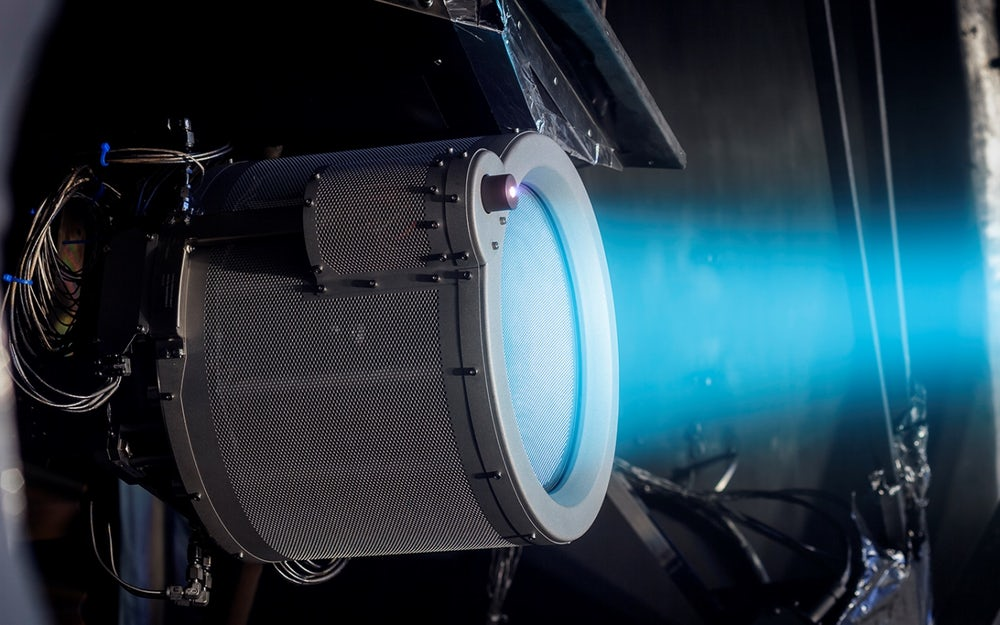
\includegraphics[width=\defaultwidth]{ion_Bepi.png}
  \caption{The T6 ion thruster will help send BepiColombo to Mercury. The neutralizing cathode is in the upper left quadrant of the thruster. (Credit\string: QinetiQ)}
  \label{fig-iongridded}
\end{figure}
 
 \paragraph{Hall Effect thrusters} use a magnetic barrier to both increase the ionization of the propellant and create the accelerating electric field.
 A detailed description of the \ac{HET} is presented in the next section.
 One cathode is used to start the discharge and neutralize the ion beam.
 Compared to GITs, \ac{HET}s need less power, hence reaching better thrust per power ratio and a smaller (therefore lighter) Power Processing Unit.
 Recently, the first satellites of two mega-constellations (OneWeb, 648 satellites planned, from which six were launched on February, \nth{26} 2019, and Starlink, 12~000 satellites planned, from which 62 were launched on May, \nth{23} 2019) were sent to Low Earth orbit, both using \ac{HET}s. 


 Their typical \Isp is of the order of 1500~s.
 \Cref{fig-13kWHET} shows a high power prototype firing.
 We see the emitting cathode, in this design at the center, and the ion beam.
 \begin{figure}[!hbt]
   \centering
   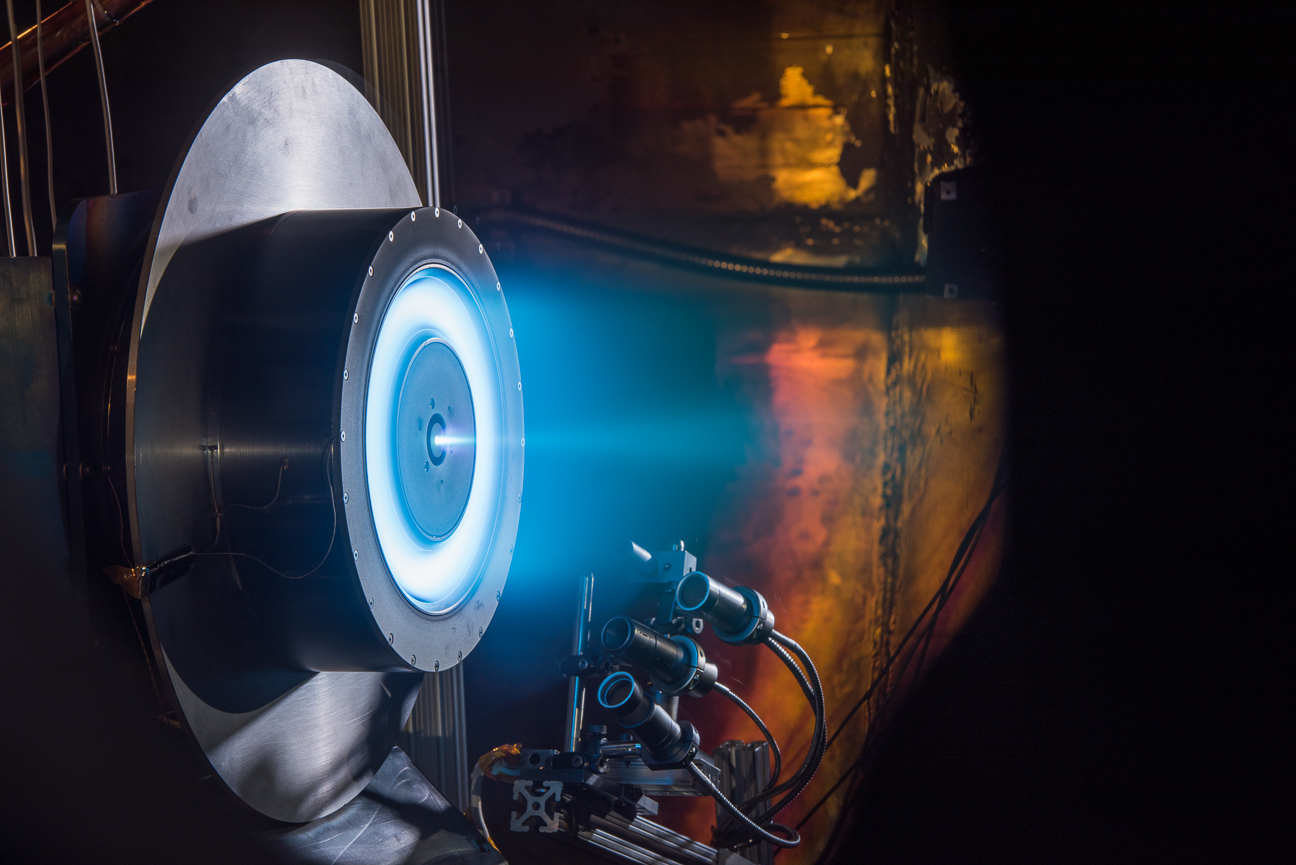
\includegraphics[width=\defaultwidth]{HET_X3_light.png}
   \caption{A 13 kilowatt \acs{HET} prototype on a testing bench in a vacuum chamber (Credit\string: NASA).  }
   \label{fig-13kWHET}
 \end{figure}
 
 
 \subsection{Electric propulsion environment in France} \label{subsec-HET_thruster}
 
 France is a leader country in the aerospace industry in both Europe and the world, with companies such as  Airbus, Thales, Safran, and ArianeGroup (join-venture of Safran and Airbus).
 As a consequence, the French ecosystem of electric propulsion is vibrant.
 The main thrusters produced in France are the PPS series by Safran, with the \PPS1350 (version G at 1.5~kW nominal power, and the version E at 2.7~kW), and the \PPS5000, a high power \ac{HET} at 5~kW, the first models of which have been delivered to Boeing in May 2019.
 A low-power version (between 500W and 1kW) of the \PPS{}  is currently developed\citep{vaudolon2018}.
 A list for the \PPS{} series elements and their respective characteristics can be seen in \cref{tab-ppsfamily}.
 \begin{table}[!hbt]
 \ra{1.3}
   \centering
   \caption{Members of the \PPS{} series developed by Safran Aircraft Engines \citep{boniface2017,duchemin2017,vaudolon2018}. The nominal operating condition of the \PPS{X00} is not fixed yet.}
   \label{tab-ppsfamily}
   \begin{tabular}{@{}llll@{}} \toprule
   Name & Power & Thrust & \Isp \\ \midrule
   \PPS1350-G & 1.5~kW & 89~mN  & 1650~s \\
   \PPS1350-E & 2.7~kW & 140~mN  & 1800~s \\
   \PPS5000 & $3-5$~kW & $150-300$~mN  & $1850-1700$~s \\
   \PPS{X00} & $\sim 650$W &  $\sim$40~mN & $\sim 1450$~s \\
   \bottomrule
   \end{tabular}
 \end{table}
 
 Several initiatives concerning the small-sat sector are also undertaken, such as the start-ups Exotrail (micro \ac{HET}) and Thrust Me (radio frequency Ion Thruster), or the Electron Cyclotron Resonance Thruster at ONERA.
 Since 1996, numerous research projects have been carried out in France on HET with  the \ac{CNES}, SAFRAN and several research laboratories: ICARE, LAPLACE, CPHT, LPP, etc. \citep{boniface2017}.
 These numerous actors, combined with the support of the French and European space agencies, compose a stimulating environment that contributes both to the most mature technologies and the promising \ac{EP} concepts that could disrupt the propulsion sector.
 
 

\section{Electric propulsion challenges}
\label{sec-challenges}
% \addcontentsline{toc}{section}{EP Industrial challenges}

Several challenges are currently tackled in the \ac{EP} industry.
The most prominent are listed by \citet{samukawa2012}\string:
\begin{enumerate}
  \item Performance improvement\string: efficiency, lifetime, and cost-effectiveness.
   Lifetime is an important issue and is limited by electrode or wall erosion.
   The lifetime of an electric thruster must be larger than 10 000 h of (reliable) operation.
   \item  Design of more versatile thrusters, i.e. able to operate at different combinations of thrust and propellant velocity.
   \item  Extension of the domain of operation to lower power ($\mu$N to 10 mN thrust range) for microsatellites or accurate attitude control.
   \item  Extension to higher power for orbit raising of telecommunication satellites (several tens of kW) and    interplanetary missions (100 kW and more).
   \item Extension of EP to low-altitude spacecraft\string: there is an increasing interest in civilian and military satellites flying  at altitudes around 100 km where the drag is significant and must be continuously compensated.
\end{enumerate}

\ac{HET} technology has the potential to answer many of these challenges.
For instance, the lifetime issue can be addressed with wall-less and magnetically shielded configurations.
Versatility is tackled with dual-mode \ac{HET} configuration \citep{boniface2017}, low power thruster is attained with $\mu$-thrusters \citep{lascombes2018}, and so forth.
However, the development of \ac{HET}s is slow and expensive. 
A better physical understanding of the processes governing \ac{HET}s is needed in order to reduce the cost and development times.
This is the objective of the current collaboration between Safran Aircraft Engines and \ac{LPP}.

\acresetall
% !TEX root=/home/tavant/these/manuscript/src/manuscript.tex

\chapter{Particle-In-Cell simulations of HETs}
\label{ch-1}

\begin{Chabstract}
  
\lipsum[1-2]

\end{Chabstract}

\minitoc


 

% !TEX root=/home/tavant/these/manuscript/src/manuscript.tex

\section{Elements of the 2D PIC-MCC simulations}
  \label{sec-elements}
  \subsection{The PIC simulations}
    \label{subsec-intro}
    The \ac{PIC} simulation models particles moving freely on a grid.
    The grid is used to compute the electric field, in the electrostatic approximation by solving the Poisson equation
    \begin{equation}
      \label{eq-poisson}
      \Delta \phi = - \frac{\rho}{\epsilon_0}
    \end{equation}
    where $\phi$ is the electric potential, $\rho$ is the charge density, and $\epsilon_0$ the vacuum permittivity.
    If the electrostatic approximation is not correct, one needs to solve the Maxwell equations.

    The particles move following the Lorentz forces
    \begin{equation}
      \label{eq-Lor}
      m \deriv{\vec{v}}{t} = q \vect{E} + q \vec{v} \times \vec{B}
    \end{equation}
    with $m$ and $q$, the particle mass and electric charge, respectively.
    The numerical particles followed in the simulations correspond to $q_f$ physical particles, with
    \begin{equation}
      q_f = \frac{n V}{\Npc}
    \end{equation}
    with $n$ the particle density, $V$ the volume of a cell, and $\Npc$ the number of numerical particles in a cell.
    A large enough number of particles is needed in order to obtain physical results.
    Indeed, an insufficient number of particles leads to numerical heating \cite{ueda1994}.
    Usually, a minimum of 100 particles per cell is used, but recent results seem to encourage to use more particles \cite{janhunen2018}.

  \subsection{The Monte Carlo collisions}

    In \ac{PIC} simulations, collisions between charged and neutral particles can be modeled by binary collision, but this approach is computationally costly.
    Instead, a Monte-Carlo algorithm can be used \cite{vahedi1995}.
    This approach is very efficient and allows scattering, momentum transfer, and ionization to be consistently modeled.
    The propellant used in \ac{HET} is \ac{Xe}.
    The cross-sections used for modeling \ac{Xe} or other gases collisions are taken from the {\sc LXCat} database project \cite{LXCat_web,pancheshnyi2012}.
    Unless otherwise stated, the elastic, inelastic scattering and ionization reactions listed in \cref{tab-reactXe} are used.
    The cross-section values are summarized in \cref{fig-xexsection}.

    \begin{table}[hbt]
      \ra{1.3}
      \centering
      \caption{Reactions for xenon used in the PIC simulations}
      \label{tab-reactXe}
      \begin{tabular}{@{}lll@{}}  \toprule
        Reaction & Threshold & Reference\\ \midrule
        {\it Elastic scattering} & &\\
        e + Xe = e + Xe   & --   & \cite{Lxcat_Xe,Lxcat_Xe2} \\
        {\it Excitation} & &\\
        e + Xe = e + Xe$^*$   & 8.315eV   & \cite{Lxcat_Xe,Lxcat_Xe2} \\
        e + Xe = e + Xe$^*$   & 9.447eV   & \cite{Lxcat_Xe,Lxcat_Xe2} \\
        e + Xe = e + Xe$^*$   & 9.917eV   & \cite{Lxcat_Xe,Lxcat_Xe2} \\
        e + Xe = e + Xe$^*$   & 11.7eV    & \cite{Lxcat_Xe,Lxcat_Xe2} \\
        {\it Ionization} & &\\
        e + Xe = e + Xe$^+$   & 12.13eV   & \cite{Lxcat_Xe,Lxcat_Xe2} \\
        \bottomrule
      \end{tabular}
    \end{table}



    \begin{figure}[hbt]
      \centering
      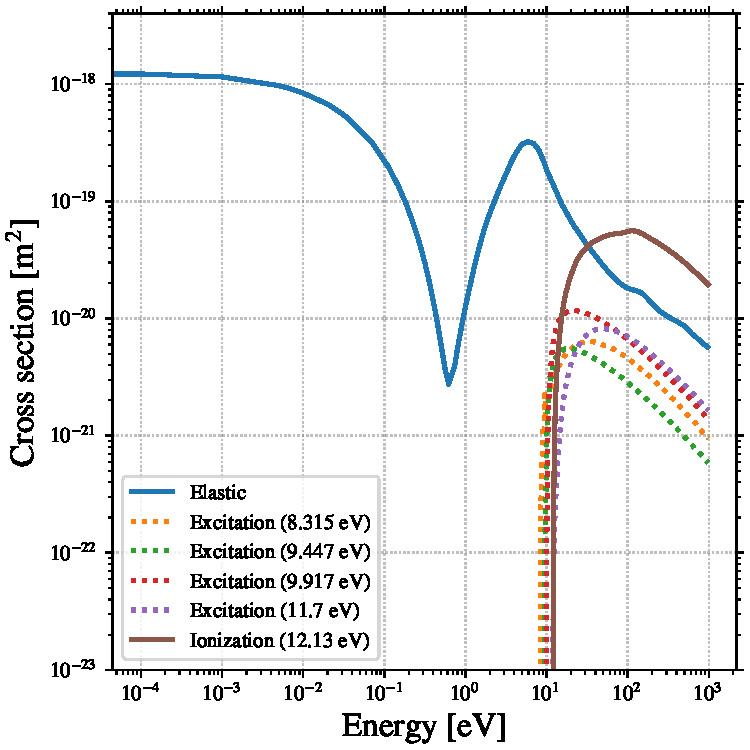
\includegraphics[width=\defaultwidth]{figure/xenon_cross_section.pdf}
      \caption{Cross section values used in the Monte Carlo procedure \cite{Lxcat_Xe,Lxcat_Xe2}.}
      \label{fig-xexsection}
    \end{figure}

    In the context of this thesis, and except precised otherwise, the `\ac{PIC} simulation' refers to the `\ac{PIC}-\ac{MCC} simulation'.
    In the case where no collision is modeled, we also call it `collisionless simulation'.



\acresetall
% !TEX root=/home/tavant/these/manuscript/src/manuscript.tex

\clearpage
\ifodd\value{page}\else
  \thispagestyle{empty}
\fi


\chapter[Study of dielectric impact on mobility]{Impact of the dielectric walls on the anomalous electron mobility }
\label{ch-2}

\begin{Chabstract}

\emph{
Part of the work presented in this chapter has been published in \citet{tavant2018}.}
\end{Chabstract}
\vspace{1ex}

\begin{Chabstract}
\lipsum[1-2]
\end{Chabstract}


\minitoc



 

\section{Presentation of the study}
  \label{sec-params}
  
  
  
  As introduced in \Cref{ch-1}, the \ac{HET} behavior depends strongly on the axial electron transport toward the anode across the magnetic barrier.
  Two main phenomena are proposed to enhance the electron mobility,
  \begin{itemize}
    \item plasma instabilities and in particular the azimuthal \ac{ECDI}, extensively studied in \cref{ch-5}
    \item the electron induced electron emission from the wall
  \end{itemize}
  In order to compare quantitatively the relative importance of the two phenomena, we propose to conduct a parametric study on the dielectric wall characteristics.
  As highlighted in the introduction and in \cref{ch-5}, the \ac{ECDI} rises due to the $E \times B$ electron drift, but saturates due to both the axial convection which limits the electron heating, and the ion-wave trapping.
  
  The first section describes the parameters of the simulation, 
  while the second section highlights the main characteristics of the base simulation results (electron mobility, plasma potential, electron mobility, etc.).
  The other sections of the chapter present the results of the parametric study on the wall characteristics\string: first we study in \cref{sec-diel_layer} the influence of the dielectric layer, then in \cref{sec-see} the secondary electron emission is analyze, and lastly we combine the two characteristics in \cref{sec-fulldiel}.

  The simulation domain corresponds to the exit plane of the thruster.
  Hence, a neutral pressure $P_n$ of 0.1~mTorr and a plasma density $n_e$ of $\sn{1}{17}$ m$^{-3}$ are used.
  The fixed axial electric field and radial magnetic field are $E_z=\sn{2}{4}\,\volt\per\meter$ and $B_r=200$ G, respectively.
  The rectangular \acs{2D} domain measures $L_r=2$~cm in the radial dimension and $L_{\theta}=0.5$~cm in the azimuthal direction.
  The axial length used for the convection is set to $L_z=1$~cm.
  It is important to note that the results shown in this chapter have been obtained at the beginning of my thesis, before the study of the convection presented in \cref{ch-1}.
  Hence, in this chapter we use the convection model of \citet{lafleur2016a}.
  However, we have validated that the convection model used does not modify the results under the conditions studied.
  The numerical parameters are chosen to respect the stability criterion of \ac{PIC} simulation, and are presented in \Cref{parameters}
  
  \begin{table}[htbp] %PIC parameters
       \centering
       \ra{1.3}
       \caption{\label{parameters} Standard operating and numerical parameters used in the 2D PIC simulations of an HET.  The simulation results are given as representative values.}
       \begin{tabular}{@{}r c c c@{}} 
          \toprule
          {\bf Physical Parameter} & notation & Value & Unit \\
          \midrule
          Gas & & Xenon & - \\
          Domain dimensions & $L_{x} \times L_{y} \times L_{z}$ & $2.0 \times 0.5 \times 1.0$ & [cm$^3$] \\
          Radial magnetic field & $B_{0}$                    & $200$                 & [{G}] \\
          Axial electric field & $E_{0}$                    & $2 \times 10^{4}$     & [{Vm}$^{-1}$] \\
          Mean plasma density & $n_{0}$                    & $3 \times 10^{17}$    & [{m}$^{-3}$] \\
          Initial electron temperature & $\Te_{,0}  $               & $10.0$                 & [{V}] \\
          Initial ion temperature & $T_{i,0}   $               & $0.1$                 & [{V}] \\
          Secondary electron temperature & $T_{see}   $               & $1.0$                 & [{V}] \\
          Neutral gas pressure & $P_{n}     $               & $1.0$                 & [{mTorr}] \\
          Neutral gas temperature & $T_{n}     $               & $300$                 & [{K}] \\
          Neutral gas density & $n_{g}     $               & $3.22 \times 10^{19}$ & [{m}$^{-3}$]\\
          \midrule
          {\bf Simulation Parameter} &  &   &  \\
          
          Time step & $\Delta t  $                      & $4 \times 10^{-12}$ & [{s}] \\
          Cell size & $\Delta x = \Delta y$ & $2 \times 10^{-5}$  & [{m}] \\
          Number of particles per cell & $N/NG      $                      & $80$                & [{part/cell}] \\
          \midrule
          {\bf Typical quantities} &  &  &  \\ 
          Electron plasma frequency & $\omega_{pe}$               & $3.1 \times 10^{10} $  & [rad/s]\\
          Ion plasma frequency & $\omega_{pi}$               & $36 \times 10^{6} $  & [rad/s]\\
          Electron cyclotron frequency & $\omega_{ce}$               &  $3.5\times 10^{9}$  & [rad/s] \\
          Electron Larmor radius & $r_{Le}$                    & 6$\times 10^{-4}$    & [m] \\
          \bottomrule
       \end{tabular}
    \end{table}
  
  
  The simulation is initialized with a uniform density of particles, following a Maxwellian distribution with temperatures $\Te_{,0}$ and $\Ti_{,0}$ for the electrons and the ions, respectively.
  
  
% !TEX root=/home/tavant/these/manuscript/src/manuscript.tex

\section{The base case}
  \label{sec-canonical}
  
  
  The {\it base} case corresponds to the case when the walls are grounded, and are fully absorbing. 
  It is the reference case that will be extensively described and commented.
  Then, it will be used as reference to analyze and quantify the effects of two characteristics of the dielectric walls on the studied discharges : the secondary electron emission, and the modification of the electrostatic boundary condition.
  
  \subsection{Initial phase of the simulation\string: \texorpdfstring{$t < 2\,\micro\second$}{ t < 2 microseconds} } \label{subsec-initlaphase}
  
  The initial phase of the simulation corresponds to the growth of the \ac{ECDI}, and the formation of the sheaths.
  Because of the growth of the instability, the electron transport increases as well, which increases the electron heating.
  The time scale of the sheath formation is governed by the ion inertia.
  It is roughly the same time scale as the saturation of the instability due to ion-trapping.
  
  \begin{figure}[hbt]
    \centering
    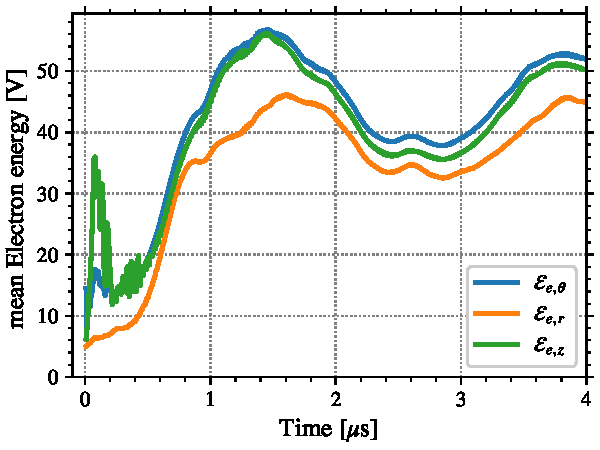
\includegraphics[width=\defaultwidth]{canonical_Te_start_directions}
    \caption{Temporal evolution of the electron mean kinetic energy decomposed over the three directions. Only the beginning of the simulation is shown.}
    \label{fig-canon_Te_strat}
  \end{figure}
  
  \Cref{fig-canon_Te_strat} shows the temporal evolution of the electron mean kinetic energy decomposed over the three directions, $\Ee_r, \Ee_{\theta}, \Ee_z$, such that
  \begin{equation} \label{eq-Ee_direction}
    \Ee_d = \frac{1}{n} \frac{1}{2} m_e \iiint_{\vect{v}}  v_{e,d}^2 f (\vect{v}) d^3v, \text{ with } d \in \{r, \theta, z  \}
  \end{equation}
  The mean kinetic energy is the sum of the thermal energy and the kinetic energy of the mean velocity.
  Because the electrons drift mainly in the azimuthal direction, we have
  \begin{equation} \label{eq-kinetic}
    \begin{cases}
      \Ee_r \simeq \frac{\Te_r}{2} \\
      \Ee_z \simeq \frac{\Te_z}{2} \\
      \Ee_{\theta} \simeq \frac{\Te_{\theta}}{2} + \frac{m_e}{2} \lp \frac{E_0}{B_0} \rp^2 \\
    \end{cases}
  \end{equation} 
  with $\frac{m_e}{2} \lp \frac{E_0}{B_0} \rp^2 \simeq  2.84\,\volt $.
  \nomenclature[Q]{\ensuremath{ \Ee}}{ Electron total kinetic energy, imposed of the thermal (or internal) energy and the kinetic energy of the mean velocity.  }
  We see that after some high frequency oscillations of $\Ee_{\theta}$ and $\Ee_z$ due to the cyclotron motion, the energies rise before stabilizing at $\Ee \simeq 45$V.
  The radial kinetic energy $\Ee_r$ is less than $\Ee_z$ and $\Ee_{\theta}$, but only by a small difference of $5\,\volt$, corresponding to roughly $10\%$.
  The small difference between the azimuthal and the axial kinetic energy is of the order of $2\,\volt$, as expected from the cyclotron motion of the electrons and \cref{eq-kinetic}.
  This means that the electrons are almost isotropic.
  
  
  \begin{figure}[hbt]
    \centering
    \begin{tabular}{@{} c c}
      \subfigure{time_r_mean_n}{a}{20, 20} &
          
      \subfigure{time_r_mean_phi}{b}{20, 20} 
    \end{tabular}
    \caption{Temporal evolution of the radial profile of the ({\bf a}) electron density and ({\bf b}) the plasma potential averaged azimuthally.}
    \label{fig-tx_n_phi}
  \end{figure}

  We can see in \Cref{fig-tx_n_phi} the evolution of the radial profile of the electron density on the plasma potential over the same period as \cref{fig-canon_Te_strat}.
  We observe on both quantities the formation of the sheath and the evolution toward a steady-state.
  
  \subsection{Saturated quasi steady-state\string: \texorpdfstring{$t \geq 2\,\micro\second$}{t > 2 microseconds}  }
  \label{subsec-stablephase}
  After the relatively fast rise of the plasma characteristics, the simulation reaches a quasi steady-state, as we can see in \Cref{fig-canon_Te_all}.
  We observe that after $t\simeq2\mus$ , the electron energy $\Ee$ starts to oscillate around a mean value.
  The oscillations are then damped and reach their minimum amplitude at  $t\simeq 7\mus$ and then remain with a small amplitude as shown on simulations carried out up to $25\,\micro\second$ in \cref{fig-canon_Te_all} (the origin of these oscillations has been discussed in \Cref{subsec-temp}).  
  
  
  \begin{figure}[hbt]
    \centering
    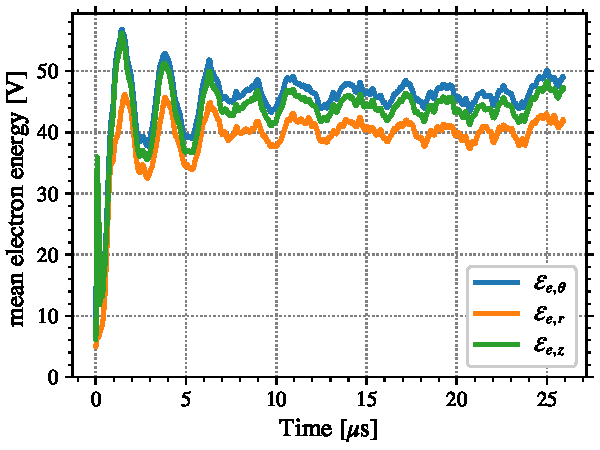
\includegraphics[width=\defaultwidth]{canonical_Te_all_directions_long}
    \caption{Temporal evolution of the electron mean kinetic energy decomposed over the three directions, similar to \cref{fig-canon_Te_strat} but for a longer period. We still see the difference between $\Ee_z$ and $\Ee_{\theta}$ due to the $E\times B$ drift, and the colder radial energy.}
    \label{fig-canon_Te_all}
  \end{figure}
  

  \Cref{fig-profiles} shows the azimuthally-averaged radial profiles of the electron and ion densities.
  The plasma is mostly quasineutral, except close to the walls, in the sheath, where the electron density falls more rapidly compared to that of ions.
  The sheath length can be roughly estimated to be $1\,\milli\meter$.
  The Debye length in our conditions is
  \begin{equation} \label{eq-debye}
    \lambda_D = \sqrt{\frac{\epsilon_0 k_b T_e}{n_e e^2}} \sim 0.4\,\milli\meter,
  \end{equation}
  which corresponds to the expected floating sheath length \citep{chabert2014} (a few $\lde$).
  
  \begin{figure}[hbt]
    \centering
    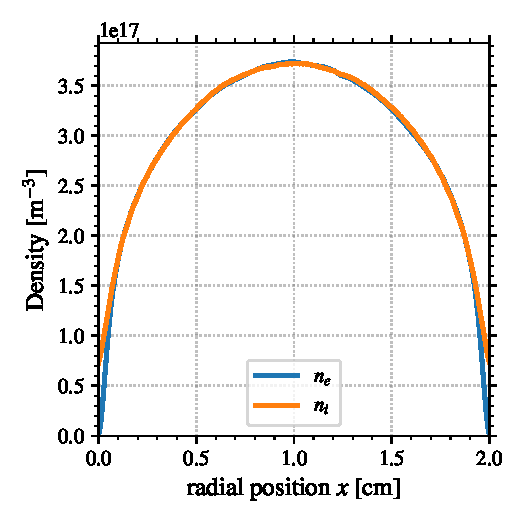
\includegraphics[width=\defaultwidth]{density_profile.pdf}
    \caption{Radial profile of the ion and electron densities at steady-state, averaged azimuthally and in time over the 5 last microseconds.}
    \label{fig-profiles}
  \end{figure}
  
  \subsection{Enhanced electron transport} \label{subsec-canonmue}
  As introduced in \cref{sec-transport}, the electron cross-field axial transport is characterized by the electron mobility
  \begin{equation} \label{eq-mobdef}
    \mobe = \frac{u_{e, z}}{E_z}
  \end{equation}
  with $u_{e,z}$ and $E_z$ the electron mean axial velocity and the axial electric field, respectively.
  \nomenclature[Q]{\ensuremath{ u_e, u_i}}{ Electron and ion mean velocities}
  In \ac{PIC} simulations, $\mobe$ is computed at each time step by
  \begin{equation} \label{eq-mobpic}
    \mobpic = \frac{1}{N E_z} \sum_N v_{e,z}
  \end{equation}

  \begin{figure}[hbt]
    \centering
    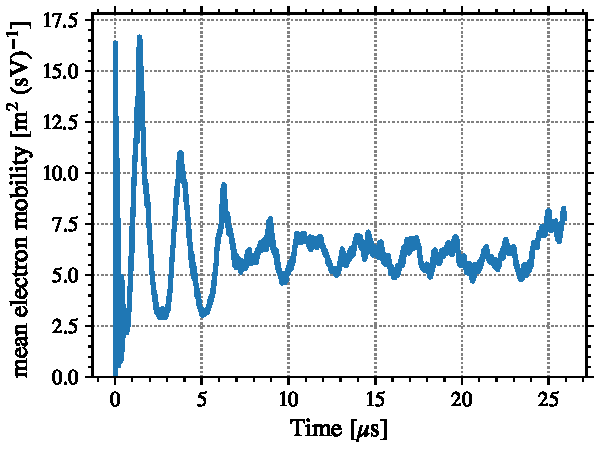
\includegraphics[width=\defaultwidth]{canonical_mu_all}
    \caption{Temporal evolution of the electron axial mobility computed in the \acs{PIC} simulation.}
    \label{fig-canon_mu}
  \end{figure}
  
  \Cref{fig-canon_mu} shows the temporal evolution of the electron mobility $\mobpic$ measured in the simulation with \cref{eq-mobpic}.
  We can see that it presents the same characteristics as the evolution of the electron energy $\Ee$ on \cref{fig-canon_Te_all}.
  We recall that the classical electron mobility from the collisional theory developed in \cref{eq-mobility} is \citep{lafleur2016a}
  \begin{equation} \label{eq-muclass}
    \mobcla = \frac{\nu_m \frac{e}{m_e}}{\oce^2 + \nu_m^2}
  \end{equation}
  with $\nu_m$ the electron-neutral  collision frequency and \oce{} is the electron cyclotron frequency.
  In the conditions of \cref{parameters}, $\mobcla \simeq 0.8$ \square\meter(sV)$^{-1}$.
  
  The measured electron mobility in the \ac{PIC} simulation is one order of magnitude larger than the classical mobility.
  In the present case, as no electron is emitted from the wall, the enhancement can only come from the instabilities present in the plasma.

  % K_ex = 2 10^-13
  % n_g = 1e19
  % wce = q B / m
  The oscillations can be seen in \cref{fig-2dschemat}, which shows the azimuthal electric field observed at $T=4\,\micro\second$.
  It clearly features the oscillation of wavelength of the order of 1~mm, as observed in \citet{heron2013}, and \citet{janhunen2018}.
  \Cref{fig-exampleECDI} shows the temporal evolution of the azimuthal electric field measured at the center of the channel.
  We can see that the instability rises and saturates quickly.
  Then, the oscillation remains quite stable.
  The Fourier Transform of the electric field presents a clear maximum at $14\,\mega\hertz$.
  The theoretical frequency of the \ac{ECDI} instability is \citep{lafleur2017}
  \begin{equation} \label{eq-maxfeq}
    f_{\rm max} = \frac{\omega_{pi}}{\sqrt{3}} \simeq 21 \,\mega\hertz,
  \end{equation}
  which gives a relatively good agreement with the oscillation observed.
  The \ac{ECDI} instability was the subject of \Cref{ch-5}, hence it will not be further discussed here.
  
  
  \begin{figure}[hbt]
    \centering
    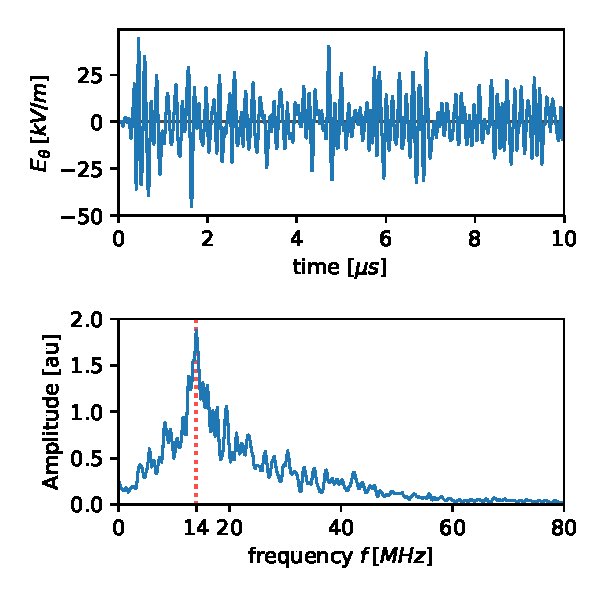
\includegraphics[width=\defaultwidth]{time_and_FFT}
    \caption{Azimuthal instability\string: temporal evolution of the azimuthal electric field at the center of the simulations, and its frequency spectrum computed by \acs{FFT}. The frequency for which the amplitude is maximum is highlighted.}
    \label{fig-exampleECDI}
  \end{figure}
  
  The effective mobility $\mobeff$ is determined by the correlation term $<\dEt \dne>$ and the parameters of the simulations.
  The effective mobility at saturation $\mobeffsat$, using the hypothesis of saturation by ion-wave trapping, only needs the electron temperature $\Te$.
  We can see that the three values $\mobpic, \mobeff$, and $\mobeffsat$ are close from each-others.
  
  \begin{table}[!hbt]
  \ra{1.3}
    \centering
    \caption{Characteristics  measured in the simulation at $t=27\,\micro\second$.}
    \label{tab-canonical_mobility}
    \begin{tabular}{@{} r l @{}} \toprule
    Quantity & Value \\ \midrule
    Correlation $<\dEt \dne>$ & $\sn{6}{20}$ V/m${^4}$ \\
    Effective mobility $\mobeff$ from \cref{eq-eq_mobeffsimple_two} & 4.4 m$^2$(sV)$^{-1}$ \\
    Mobility saturation $\mobeffsat$ from \cref{eq-mobeffsat} & 3.3 m$^2$(sV)$^{-1}$ \\
    Measured mobility $\mobpic$ from \cref{eq-mobpic} & 6 m$^2$(sV)$^{-1}$\\
    \bottomrule
    \end{tabular}
  \end{table}
  

  
  

\acresetall
% !TEX root=/home/tavant/these/manuscript/src/manuscript.tex
\clearpage
\ifodd\value{page}\else
  \thispagestyle{empty}
\fi
\chapter{Conclusion}
\label{ch-conclusion}

\headerchaptername{Conclusion}

\section{Summary of the thesis}

  \lipsum[1-2]

  \subsection{Growth and saturation of the azimuthal instability}

    \lipsum[1-2]

  \subsection{Impact of the wall characteristics on the plasma-wall interaction }
  \lipsum[1-2]



\appendix

% !TEX root=/home/tavant/these/manuscript/src/manuscript.tex

\chapter{Scalability tests}
\label{an-scalability}

\renewcommand\chaptername{Annexe}

In this annexe, we give more information on the scalability tests conducted.
We conducted both a weak and a strong scalability tests.
We recall that the strong scalability keeps the load constant while increasing the computational performance, here the number of CPU.
The weak scalability keeps the load to the number of CPU ratio constant.
However, it does not correspond to the need we had, which is to find the optimal number of CPU for a given task.
Beside, the results of the weak scalability were less clear to analyze.
Hence, we discarded them.

The parameters of the strong scalability test used are given in \cref{parameters-strong-scalability}.
They are close to the parameter used in production, presented in \cref{parameters}.
The smaller test-case uses the same settings, except for the domain which is divided by a factor of 4.
The dielectric boundary conditions are not modeled (no \ac{SEE}, no dielectric layer).
The Inputs, set-up, and Outputs are not taken into account in the study of the performances.
However, the usual diagnostics (mean density, fluxes, temperature, at boundaries and in the plasma) are computed.
The performances are averaged over the 1000 first time steps of the simulations.
Hence, the load is well balanced between the CPU. 


\begin{table}[htbp] %PIC parameters
     \centering
     \ra{1.3}
     \caption{\label{parameters-strong-scalability} Operating and numerical parameters used in the strong scalability large test-case.}
     \begin{tabular}{@{}r c c c@{}} 
        \toprule
        {\bf Physical Parameter} & notation & Value & Unit \\
        \midrule
        Gas & & Xenon & - \\
        Domain dimensions & $L_{x} \times L_{y}$ & $1.0 \times 1.023$ & [cm$^2$] \\
        Radial magnetic field & $B_{0}$                    & $200$                 & [{G}] \\
        Axial electric field & $E_{0}$                    & $2 \times 10^{4}$     & [{Vm}$^{-1}$] \\
        Mean plasma density & $n_{0}$                    & $1 \times 10^{17}$    & [{m}$^{-3}$] \\
        Initial electron temperature & $\Te_{,0}  $               & $1.0$                 & [{V}] \\
        Initial ion temperature & $T_{i,0}   $               & $0.05$                 & [{V}] \\
        Neutral gas pressure & $P_{n}     $               & $0.1$                 & [{mTorr}] \\
        Neutral gas temperature & $T_{n}     $               & $300$                 & [{K}] \\
        Neutral gas density & $n_{g}     $               & $3.22 \times 10^{18}$ & [{m}$^{-3}$]\\
        \midrule
        {\bf Simulation Parameter} &  &   &  \\
        
        Time step & $\Delta t  $                      & $4 \times 10^{-13}$ & [{s}] \\
        Cell size & $\Delta x = \Delta y = \Delta z $ & $5 \times 10^{-7}$  & [{m}] \\
        Number of particles per cell & $N/NG      $                      & $150$                & [{part/cell}] \\
        Number of particles & $N      $                      & $2 \times 614099924$                & [{particles}] \\
        
        Number of time steps & $N_t$ & 1000 & --\\
        
        
        \bottomrule
     \end{tabular}
  \end{table}
  
  \begin{table}[hbt]
  \ra{1.3}
    \centering
    \caption{Modified parameter for the strong-scalability small test-case. The other parameters are given in \cref{parameters-strong-scalability}. }
    \label{tab-peremeters-small}
    \begin{tabular}{@{}r c c c@{}} 
      \toprule
      {\bf Physical Parameter} & notation & Value & Unit \\
      \midrule
      Domain dimensions & $L_{x} \times L_{y}$ & $1.0 \times 1.023$ & [cm$^2$] \\
      \midrule
      {\bf Simulation Parameter} &  &   &  \\
      Cell size & $\Delta x = \Delta y = \Delta z $ & $1 \times 10^{-6}$  & [{m}] \\
    \bottomrule
    \end{tabular}
  \end{table}
  
  An example of the relative importance of each module of the simulation over a time step is given in \cref{tab-example_perf}.
  Each module is called 1000 times, except for the outputs function, that writes the diagnostics to the disk, which is called only once.
  Its duration is divided by the number of time steps, in order to compare it to the other modules.
  To give an order of magnitude, taking $t=10.08\,\second$ for one time-step corresponds to an average of $8.2\,\nano\second$ per particle.
  
  \begin{table}[hbt]
  \ra{1.3}
    \centering
    \caption{Performances of the large test-case (parameters of \cref{parameters-strong-scalability}) when using 96 CPUs, average over 1000 time steps. }
    \label{tab-example_perf}
    \begin{tabular}{@{}r c c@{}} 
      \toprule
    Module  & Duration one time-step [s]  & Percentage \\
    \midrule
    Total & 10.08 & 100 \\
    Diagnostics particle to mesh & 6.03 & 59.9 \\
    Particle motion & 2.88 & 28.6 \\
    Monte Carlo Collision & 0.729 & 7.31 \\
    Outputs & 0.287 & 2.84 \\
    Poisson solver & 0.075 & 0.75 \\
    \bottomrule
    \end{tabular}
  \end{table}
  


\backmatter

\markboth{BIBLIOGRAPHY}{}

\renewcommand{\bibname}{\label{ch-bibliography}Bibliography}

\bibliographystyle{unsrtnatperso}  
% \bibliographystyle{theseen-nat-href}  
\bibliography{bib/bibliography}


% !TEX root=/home/tavant/these/manuscript/src/manuscript.tex

% 
% 
\cleardoublepage

\checkoddpage
\ifoddpage
  \null\newpage
  \thispagestyle{empty}

  \else 
  %nothing
\fi



\pagestyle{empty}

%% Logo de l'école doctorale. Le nom du fichier correspond au sigle de l'ED / Doctoral school logo. Filename correspond to doctoral school acronym
%% Les noms valides sont / Valid names are \string: 2MIB; AAIF; ABIES; BIOSIGNE; CBMS; EDMH; EDOM; EDPIF; EDSP; EOBE; INTERFACES; ITFA; PHENIICS; SDSV; SDV; SHS; SMEMAG; SSMMH; STIC
\begin{textblock*}{61mm}(16mm,3mm)
	\noindent\includegraphics[height=24mm]{couvertures/ed/\logoEd.jpeg}
\end{textblock*}
\topskip=0pt  %\offinterlineskip 

\vspace*{0em}


%%%Titre de la thèse en français / Thesis title in french
\setlength\fboxsep{3mm}
\begin{center}
\fcolorbox{bordeau}{white}{\parbox{0.99\textwidth}{
{\large {\bf Titre\string:} \PhDTitleFR }

\smaller
\vspace{1em}
%%%Mots clés en français, séprarés par des ; / Keywords in french, separated by ;
{\bf Mots clés\string:} \keywordsFR
\vspace{-2mm}

%%% Résumé en français / abstract in french
\begin{multicols}{2}
{\bf Résumé\string:}

\abstractFR
\end{multicols}
}}
\end{center}
\vspace*{0mm}
% 
%%%Titre de la thèse en anglais / Thesis title in english
\begin{center}
  \normalsize
\fcolorbox{bordeau}{white}{\parbox{0.99\textwidth}{
{\large {\bf Title\string:} \PhDTitleEN}

\smaller
\vspace{1em}
%%%Mots clés en anglais, séprarés par des ; / Keywords in english, separated by ;
{\bf Keywords\string:}  \keywordsEN %%3 à 6 mots clés%%
\vspace{-2mm}
\begin{multicols}{2}

%%% Résumé en anglais / abstract in english
{\bf Abstract\string:}
\abstractEN

\end{multicols}

}}
\end{center}
% 
\textblockcolour{white}
% \begin{textblock*}{161mm}(10mm,270mm) % uncomment for A4
\begin{textblock*}{161mm}(10mm,230mm) % uncomment for B5
%
\color{bordeau}
{\bf\noindent Université Paris-Saclay	         }

\noindent Espace Technologique / Immeuble Discovery

\noindent Route de l’Orme aux Merisiers RD 128 / 91190 Saint-Aubin, France
\end{textblock*}

\textblockcolour{white}

% \begin{textblock*}{20mm}(180mm,253mm) % uncomment for A4
\begin{textblock*}{20mm}(140mm,223mm) % uncomment for B5


\includegraphics[width=20mm]{couvertures/UPSACLAY-petit}
\end{textblock*}



\end{document}


% Resources:

% floats (tables, figures, etc.
% https://tex.stackexchange.com/questions/2275/keeping-tables-figures-close-to-where-they-are-mentioned
% http://tug.ctan.org/tex-archive/info/epslatex/english/epslatex.pdf
% https://tex.stackexchange.com/questions/39017/how-to-influence-the-position-of-float-environments-like-figure-and-table-in-lat/39020#39020

